%% LyX 2.3.2-2 created this file.  For more info, see http://www.lyx.org/.
%% Do not edit unless you really know what you are doing.
\documentclass[12pt,british,UKenglish]{article}
\renewcommand{\rmdefault}{ptm}
\usepackage[T1]{fontenc}
\usepackage[latin9]{inputenc}
\usepackage[a4paper]{geometry}
\geometry{verbose,tmargin=2cm,bmargin=2cm,lmargin=2.5cm,rmargin=2.5cm}
\setlength{\parskip}{\medskipamount}
\setlength{\parindent}{0pt}
\usepackage{color}
\usepackage{array}
\usepackage{longtable}
\usepackage{tabularx}
\usepackage{booktabs}
\usepackage{enumitem}
\usepackage{calc}
\usepackage{pdfpages}
\usepackage{amsmath}
\usepackage{tikz}
\usetikzlibrary{positioning, arrows.meta}
\usepackage{amssymb}
\usepackage{nomencl}
% APA 7th referencing; loaded before LyXPreamble so it can skip the cite package
\usepackage[style=american]{csquotes} % APA uses double quotation marks
\usepackage[backend=biber,style=apa]{biblatex}
\DeclareLanguageMapping{british}{british-apa}
\DeclareLanguageMapping{UKenglish}{british-apa}
% allow long URLs in the reference list to break at any character
\setcounter{biburlnumpenalty}{100}
\setcounter{biburlucpenalty}{100}
\setcounter{biburllcpenalty}{100}
% the following is useful if no old nomencl.sty package
\providecommand{\printnomenclature}{\printglossary}
\providecommand{\makenomenclature}{\makeglossary}
\makenomenclature

\newcommand{\fillin}[1]{\textcolor{red}{[#1]}}

%% ---- Nomenclature entries ----
\nomenclature{$\rho$}{Water density (kg/m$^3$)}
\nomenclature{$V$, $U$}{Tow speed (m/s)}
\nomenclature{$S$}{Foil planform area (m$^2$)}
\nomenclature{$C_L$, $C_D$}{Lift and drag coefficients}
\nomenclature{$L$}{Hydrodynamic downforce from the foil (N)}
\nomenclature{$D$}{Drag (N)}
\nomenclature{$B$}{Buoyancy force (N)}
\nomenclature{$W$}{Weight of the rig in air (N)}
\nomenclature{$T$}{Tow rope tension (N)}
\nomenclature{$\gamma$}{Rope angle below horizontal at the rig ($^\circ$)}
\nomenclature{$d_L$, $d_T$, $d_D$, $d_B$}{Moment arms of lift, tension, drag and buoyancy about the CoM (m)}
\nomenclature{$\alpha_{L0}$}{Zero-lift angle of attack ($^\circ$)}
\nomenclature{$\theta$}{Pitch angle, positive nose-up ($^\circ$)}
\nomenclature{$\theta_r$}{Rope angle toward which the rope pulls the body ($^\circ$)}
\nomenclature{$\theta_{\mathrm{ref}}$}{Pitch reference from the outer loop ($^\circ$)}
\nomenclature{$\phi$}{Roll angle ($^\circ$)}
\nomenclature{$\delta$}{Fin deflection ($^\circ$), limited to $\pm25^\circ$}
\nomenclature{$\beta_i$}{Mounting angle of ultrasonic beam $i$ from vertical ($^\circ$)}
\nomenclature{$r_i$}{Range reported by ultrasonic beam $i$ (mm)}
\nomenclature{$h$, $\hat h$}{Altitude above the seabed and its Kalman estimate (mm)}
\nomenclature{$h_{\mathrm{sp}}$}{Altitude set point (mm)}
\nomenclature{$k_\delta$}{Pitch-rate gain of the fins ((deg/s)/deg)}
\nomenclature{$\tau_r$}{Rope restoring time constant (s)}
\nomenclature{$K_p$, $K_i$}{Outer-loop gains (deg/mm, deg/(mm\,s))}
\nomenclature{$K_\theta$}{Inner-loop gain (deg/deg)}
\nomenclature{$Re$, $Fr$}{Reynolds and Froude numbers}
\nomenclature{$c$}{Speed of sound in water (m/s)}

\makeatletter

%%%%%%%%%%%%%%%%%%%%%%%%%%%%%% LyX specific LaTeX commands.
%% Because html converters don't know tabularnewline
\providecommand{\tabularnewline}{\\}
%% A simple dot to overcome graphicx limitations
\newcommand{\lyxdot}{.}


%%%%%%%%%%%%%%%%%%%%%%%%%%%%%% Textclass specific LaTeX commands.
\newlength{\lyxlabelwidth}      % auxiliary length 

%%%%%%%%%%%%%%%%%%%%%%%%%%%%%% User specified LaTeX commands.
\input{LyXPreamble} % import additional settings from this file

\makeatother

\usepackage{babel}
\usepackage{listings}
\lstset{basicstyle={\ttfamily\footnotesize},
belowcaptionskip=3mm,
breaklines=true,
commentstyle={\color[rgb]{0,0.5,0}},
frameshape={{NYN}{nnn}{nnn}{NYN}},
keywordstyle={\color{blue}},
language=Matlab,
numbers=left,
numberstyle={\scriptsize},
showstringspaces=false,
stringstyle={\color{purple}}}
\def\eqdeclaration#1{, see equation\nobreakspace(#1)}
\def\pagedeclaration#1{, page\nobreakspace#1}
\def\nomname{Nomenclature}
\renewcommand{\lstlistingname}{Listing}

\begin{document}
% Define your name and report number here. It will update on all pages where they are needed.
\def \name{Alex Kerr}
\def \reportNumber{ME-\the\year}

%% -
%%  Title page of the report -
%% -
\thispagestyle{empty}
\pagenumbering{roman}
% Change default name for code environments
\renewcommand\lstlistingname{Program}  

\vspace*{10mm}

\begin{center}
\textbf{\large{}Research Project in Mechatronics Engineering}{\large\par} % UPDATE this to match your specialisation
\par\end{center}

\vspace*{10mm}

\HRule
\begin{center}
Design Research Report
\par\end{center}

\begin{center}
\textbf{\Large{Automated Detection and Geolocation of Caulerpa Using an Embedded Vision System}}{\Large\par}
\par\end{center}

\begin{center}
{\large{}\name}{\large\par}
\par\end{center}

\begin{center}
Project Report \reportNumber
\par\end{center}

\HRule

\vspace*{\fill}

\begin{center}
\begin{tabular}{rl}
Co-worker: & {Rhys Chittenden}\tabularnewline   % ADD your partner's name here
\noalign{\vskip1.5em}
Supervisor: & Dr {Henry Williams}\tabularnewline    % ADD your supervisor's name here
\noalign{\vskip1.5em}
\end{tabular}
\par\end{center}

\vspace*{\fill}

\begin{center}
\cleanlookdateon \today
\par\end{center}

\vspace*{\fill}

\begin{center}
\includegraphics[width=0.7\linewidth]{Figures/mech-horizontal-hc}
\par\end{center}

\newpage{}
%% -
%%  Frontmatter of the report 
%% -

%% - ABSTRACT 
\begin{flushleft}
\reportNumber
\par\end{flushleft}

\vspace{1em}

\begin{center}
\textbf{\textsc{\large{Automated Detection and Geolocation of Caulerpa Using an Embedded Vision System}}}{\large\par}
\par\end{center}

\vspace{2em}

\begin{center}
\textbf{\large{}\name}{\large\par}
\par\end{center}

\vspace{2em}

\begin{center}
\textbf{\textsc{\large{}ABSTRACT}}{\large\par}
\par\end{center}

Invasive \textit{Caulerpa} species are spreading along the New Zealand coastline, and monitoring currently relies on diver surveys that are slow, costly and expose divers to risk. This report describes the design and testing of a low-cost, predominantly 3D-printed towed camera platform that holds a set altitude above the seabed as the carrier for Caulerpa imaging. The rig uses an inverted NACA 5518 hydrofoil for downforce, servo-driven fins for altitude control, eight ultrasonic transducers for altitude and forward ranging, and an IMU for attitude.

A 1/7th-scale Froude-matched model confirmed the passive diving response. Full-scale pool trials showed that trim is highly sensitive to the chordwise position of the tow point relative to the centre of mass, and that a single-loop PID controller from altitude error to fin angle drives the rig into sustained oscillation, because fin angle sets pitch rate and the plant behaves as a double integrator. A software-in-the-loop simulation that runs the unchanged firmware against a towed-foil model was used to redesign the controller as a cascaded PI altitude loop around a proportional pitch loop, with a Kalman altitude estimate. The simulation also showed that holding trim against the rope consumes most of the $\pm25^\circ$ fin range, and that the $35^\circ$ beams look 0.70\,m ahead at the 1\,m target, under 1.5 sonar sweeps at 1\,m/s. In pool trials at 1\,m/s the cascaded controller held the rig within the 0.5-1.5\,m band for \fillin{X}\% of the run and to \fillin{Y}\,mm RMS about the 1\,m target, against \fillin{Z}\% and \fillin{W}\,mm with the fins fixed. These results show how well hobby-grade actuation and ultrasonic sensing hold survey altitude in calm water, and identify fin authority and forward sensing range as the limits to resolve before open-water trials.
% end of Abstract

%% - DECLARATION -
\includepdf[pagecommand=\thispagestyle{fancy}]{Declaration} % Overwrite the PDF in the root folder to update with the signed document.
    

\newpage{}
%%  TABLE OF CONTENTS -
\setlength{\parskip}{6pt}
\renewcommand{\contentsname}{\large{Table of Contents}}

\tableofcontents{}

\newpage{}

\setlength{\parskip}{9pt}
%% - ACKNOWLEDGMENTS -
\section*{Acknowledgements}
\addcontentsline{toc}{section}{Acknowledgements}
\label{sec:Acknowledgements1}

I would like to express my gratitude to Brook and the rest of the team at Commercial Dive Specialists for sponsoring this engineering project. Their practical industry insight, resources and technical knowledge were needed for defining the operational scope and functional requirements of the underwater tow camera system.

I extend my deepest appreciation to my supervisor, Dr Henry Williams, for his continuous guidance, academic support and technical insight throughout this project. His advice in directing the methodology, refining the system design and providing constructive feedback was essential to the development throughout this project.

I would like to acknowledge Rhys. His shared contributions to the design of the hydrofoil shape and control algorithm made this project possible.

I would finally like to thank Isaac and Corban. Their sibling project based on the vision model helped shape the constraints through their literature readings. They also helped with testing and debugging when problems arose. 


\newpage{}
%% - GLOSSARY -
\section*{Glossary of Terms \addcontentsline{toc}{section}{Glossary of Terms}}

\begin{longtable}[l]{>{\raggedright}p{0.25\textwidth}>{\raggedright}p{0.7\textwidth}}
Altitude & Height of the rig above the seabed or pool floor. This is the controlled quantity throughout this report.\tabularnewline
Depth & Distance of the rig below the water surface. Used only where the surface is the reference.\tabularnewline
Bridle & The V-shaped pair of rope legs joining the two end-cap attachment points to the single tow rope.\tabularnewline
Downforce & Hydrodynamic force from the inverted foil acting toward the seabed.\tabularnewline
Fragmentation & Reproduction of Caulerpa from broken pieces of the plant.\tabularnewline
Look-ahead distance & Horizontal distance ahead of the rig at which a beam meets the seabed.\tabularnewline
Planform area & Area of the foil projected onto the plane of the span and chord.\tabularnewline
Time-in-band & Fraction of a run during which altitude stays within a stated band.\tabularnewline
Trim & Steady pitch attitude, and the fin angle needed to hold it.\tabularnewline
\addlinespace
\end{longtable}

\addtocounter{table}{-1}
%% - ABBREVIATIONS -
\section*{Abbreviations\addcontentsline{toc}{section}{Abbreviations}}

\begin{longtable}[l]{>{\raggedright}p{0.25\textwidth}>{\raggedright}p{0.7\textwidth}}
APF & Artificial potential field\tabularnewline
ASA & Acrylonitrile styrene acrylate\tabularnewline
BMS & Battery management system\tabularnewline
CFD & Computational fluid dynamics\tabularnewline
CoM & Centre of mass\tabularnewline
CSV & Comma-separated values\tabularnewline
DVL & Doppler velocity log\tabularnewline
IMU & Inertial measurement unit\tabularnewline
LiPo & Lithium polymer\tabularnewline
PETG & Polyethylene terephthalate glycol\tabularnewline
PI, PID & Proportional--integral, proportional--integral--derivative\tabularnewline
PoE & Power over Ethernet\tabularnewline
RMS & Root mean square\tabularnewline
ROV & Remotely operated vehicle\tabularnewline
SPI & Serial peripheral interface\tabularnewline
UART & Universal asynchronous receiver--transmitter\tabularnewline
USBL & Ultra-short baseline (acoustic positioning)\tabularnewline
VFF & Virtual force field\tabularnewline
\addlinespace
\end{longtable}

\addtocounter{table}{-1}
%% - NOMENCLATURE -
\printnomenclature{}\label{nomenclature}

\clearpage{}

\setlength{\parskip}{9pt}

\pagenumbering{arabic}

%% -
%%  Main Body of the report 
%% -

\section{Introduction}

\subsection{Problem}
Caulerpa is a type of algae found underwater, with many species classed as a highly invasive pest in coastal ecosystems. In New Zealand, \textit{Caulerpa brachypus} and \textit{Caulerpa parvifolia} were first detected at Aotea Great Barrier Island in 2021 and have since spread to further sites along the north-eastern coast \parencite{mpi_caulerpa,auckland_caulerpa}. Once established, these algae form dense layers across the seafloor, out-competing previous species and disrupting the ecological balance. This leads to a range of negative effects, including reduced diversity, altered habitats, and depletion of food sources for native marine organisms. This is estimated to cause 9.4 billion dollars of damages over the next 30 years \parencite{9.4RNZ}. 

\begin{figure}[ht]
    \centering
    \includegraphics[width=0.5\linewidth]{Figures/Caulerpa_over_coral.jpg}
    \caption{\textit{Caulerpa} covering coral.}
    \label{fig:Caulerpa}
\end{figure}

\noindent
The rapid spread of Caulerpa is especially problematic due to its ability to reproduce through fragmentation, allowing even small pieces to establish new colonies. Natural control mechanisms are limited, and human intervention is currently the primary method of containment and removal. Efforts to mitigate the spread typically involve hand removal by divers, targeted salt attacks, suction dredging, or benthic mats \parencite{niwa_caulerpa}.

While effective on a small scale, relying on divers to monitor and remove the weed is both inefficient for time and resources. It also presents safety risks and introduces a factor of human error into the success rate, and due to fragmentation, if some Caulerpa is not mapped and identified, it could grow and disrupt local ecosystems. As the infestation expands, there is a growing need for scalable, efficient, and cost-effective methods to detect and track Caulerpa locations. This challenge has motivated industry stakeholders, including Commercial Dive Specialists, to seek technological innovations that can enhance current monitoring practices.

\subsection{Project Topic}
This project investigates the feasibility of developing an autonomous or semi-autonomous tow camera system for marine surveying applications. The primary objective is to design a system capable of maintaining a consistent distance from the seafloor while preserving a parallel orientation to ensure high-quality image capture. Achieving this requires robust sensing and control strategies to account for environmental disturbances such as currents, variable seabed topology, and towing dynamics.

In addition to maintaining stable positioning, the system must incorporate obstacle detection and avoidance capabilities to prevent collisions with underwater structures or terrain. The integration of sensors, control algorithms, and mechanical design is therefore critical to the success of the system.

By enabling continuous, large-area surveying without the need for constant diver intervention, such a system has the potential to significantly improve the efficiency and safety of Caulerpa monitoring. Furthermore, it provides a platform for scalable data collection, which could support more advanced analysis techniques such as automated image classification and long-term ecological monitoring.

\subsection{Aims and Objectives}
The aim is to determine whether a low-cost, 3D-printed towed rig with hobby-grade actuation and ultrasonic sensing can hold the altitude and attitude needed for Caulerpa imaging. The objectives are to:
\begin{enumerate}[itemsep=1pt]
    \item Derive quantitative design specifications from the survey task and the literature.
    \item Design and fabricate a towed body that dives passively and is stable in yaw and roll.
    \item Integrate ultrasonic altitude and forward ranging, an IMU, and fin actuation on a tethered power and data system.
    \item Develop and tune an altitude controller using pool trials and a simulation identified from logged data.
    \item Measure altitude-holding, obstacle clearance and control authority against a fins-fixed baseline.
\end{enumerate}

\section{Literature Review}
Towed cameras are the established tool for large-area benthic surveys because they trade the manoeuvrability of an ROV for coverage, power efficiency and cost. \textcite{lembke_cbass} report that ROVs scale poorly. They are limited by battery life, optimised for exploration rather than cruising, they require skilled pilots, hold lines badly, and are expensive. Drop and stationary cameras are cheap but give point samples only. Towed platforms have simple orientation, shallow-water capability, low power draw and high area coverage, which makes them the practical choice when large areas are under constant monitoring \parencite{raoult,lembke_cbass}. Within towed systems, the distinguishing variable is how altitude above the seabed is held.
 
\begin{table}[htbp]
\centering
\footnotesize
\caption{Towed platform classes and how each holds altitude.}
\begin{tabular}{@{}>{\raggedright\arraybackslash}p{22mm}>{\raggedright\arraybackslash}p{28mm}>{\raggedright\arraybackslash}p{45mm}>{\raggedright\arraybackslash}p{45mm}@{}}
\toprule
\textbf{Class} & \textbf{Altitude mechanism} & \textbf{Strengths} & \textbf{Limitations} \\
\midrule
Skid or sled & Direct contact with the seabed & Simple, passive, altitude fixed by geometry & Disturbs the habitat being surveyed; fails on soft or rough ground \\
\addlinespace
Bottom-tending sled & Buoyancy or counterweight suspension with a trailing chain & Stable standoff with a light contact footprint & Still contacts the seabed; chain disturbs sediment and biota \\
\addlinespace
Flying (non-contact) & Distance sensor plus active control through fins, foils or thrusters & No seabed contact, consistent over varied terrain, better current tolerance & Harder to set up and operate; requires sensing and control \\
\bottomrule
\end{tabular}
\end{table}
 
\textcite{sheehan} compared these classes directly and found that bottom-sliding systems produced shakier imagery and greater seabed impact, while flying vehicles performed more consistently across varied terrain.  Flying vehicles had significantly lower seabed impact, and tolerated tidal currents better, at the cost of harder setup. Sheehan et al.\ used a flying platform with a bottom-contacting drag chain, so a fully non-contact system would have lower impact. This is necessary for Caulerpa, a contacting sled drags through the exact fragmenting algae being mapped, which disturbs the data and risks spreading the weed, and rules out pole-dragging designs such as the Pepe drifting video system \parencite{pepe}. Commercial non-contact rigs such as the SeaVu Seeker Deepscope capture stable imagery on a towed rope, but carry no forward sensing and remain exposed to collision \parencite{seavu}.
 
\subsection{Reported Operating Envelopes}
\label{tow_class}
 
\textcite{lembke_cbass} report tow speeds of 1 - 2\,m/s at 1 - 5\,m altitude, with accurate results at 2 - 3.5\,m and 1.5 - 2\,m/s, holding ideal altitude 60 - 80\% of the time and an acceptable 1 - 4\,m band 88 - 94\% of the time. That creates a performance baseline, as a controller that cannot beat roughly 60 - 80\% time-in-band offers nothing over an existing passive platform. \textcite{cresswell} benchmark an unassisted tow camera against diver-held transects. Tracking distance varied more than diver-held cameras, both vertically and laterally, and camera angle changed what was detected, with vertical orientation favouring turf algae and forward-facing video favouring erect organisms. That is directly relevant, since Caulerpa forms low continuous mats and therefore needs a near-vertical angle and a tightly held altitude. They also note that holding a vessel below 2 knots is difficult in rough conditions, and that transects were repeated two to four times for adequate coverage, which erodes the cost advantage over diver survey. The coverage advantage of towed survey is proven; what limits data quality is altitude and attitude variance, and what limits operational cost is repeated transects and equipment loss.
 
% ============================================================
\subsection{Towfish and Tow Cable Dynamics}
% ============================================================
\label{tow_force}
A towed body differs from a self-propelled vehicle in one respect that governs the whole design: the cable supplies the forward force, so the vehicle shapes its trajectory only through hydrodynamic reaction.
 
The standard simplified force set comprises cable tension acting along the cable and creating a moment about the attachment point, drag opposing motion, buoyancy set by displaced volume and material density, and reaction forces from control surfaces and body geometry \parencite{forces}. These act at different centres, so the separations between centre of gravity, centre of buoyancy, centre of pressure and attachment point produce the moments that set trim. The full description requires the six-degree-of-freedom formulation for submerged vessels established by \textcite{gertler}. For a passively stabilised body the practical simplification is to make yaw and roll self-correcting and treat depth control as a planar pitch problem.
 
The cable is not a passive tether. Studies of controllable towed systems show that cable length, diameter and scope dominate the achievable depth envelope, and that cable drag and catenary shape alter the effective tow angle at the body \parencite{controllable2005,dynamics2000}. They confirm that actuated towed systems reach substantially better depth control than passive equivalents across a range of body sizes and cable configurations. The consequence for a shallow-water rig is that tow force must be treated as an estimated, varying disturbance rather than a known input.
 
Control authority comes from generating downwards lift against that tension. A depressor is an aerofoil section set at negative incidence for this purpose and is standard equipment for holding towfish depth \parencite{depressor}. Work on adjustable hydrofoils shows that active fin control maintains stable operation across a wider range of conditions than fixed geometry, while identifying the central trade-off: shapes optimised purely for low drag lose control authority \parencite{hydrofoil}. That points away from the submarine-like hulls common in deeper-water towfish \parencite{controllable2005,dynamics2000,hydrofoil}. A Caulerpa rig runs at the slow end of the speed range, because imaging and downstream detection favour low ground speed, and control authority scales with the square of flow velocity, so it needs planform area and responsive surfaces rather than a low-drag body.
 
% ============================================================
\subsection{Depth and Roll Control}
% ============================================================
 \label{depth_lit}
The literature converges on fin actuation regulated by feedback on measured altitude. 
 
Actuator choice follows from the force balance above. A propeller or reaction wheel works against a cable tension it cannot change, and cannot remove slack from the cable. Control surfaces instead redirect the flow the tow already supplies, converting forward velocity into vertical force at negligible power cost, which is the configuration used across the controllable-towed-system literature \parencite{controllable2005,dynamics2000,hydrofoil} and suits a rig drawing from a surface supply.
 
Several design choices shrink the problem before any controller is written: symmetry about the vertical plane to suppress yaw and roll coupling, a streamlined profile to limit drag-induced oscillation, and a centre of mass well below the centre of buoyancy for a strong righting moment. With yaw and roll handled passively, active control reduces to a single axis in which fin pitch modulates lift and drag to set depth, which is what makes a low-cost implementation feasible.
 
PID dominates towed-body depth regulation on grounds of simplicity, robustness and low computational cost, and is adequate near a linear operating point. Its weakness here is the disturbance profile: tow force varies with vessel speed and sea state, seabed altitude changes as terrain passes beneath, and plant gain varies with the square of flow velocity. The adjustable-hydrofoil work addresses part of this by scheduling fin geometry rather than only the commanded angle \parencite{hydrofoil}. A PID inner loop with gain scheduling on measured tow speed retains the implementation simplicity while covering the dominant nonlinearity. What the control literature does not settle is the interaction between altitude tracking and avoidance: terrain following commands descent toward the seabed, avoidance commands ascent.
 
% ============================================================
\subsection{Underwater Sensing and Navigation}
% ============================================================
\label{sensor_lit}
Acoustic sensing is the only modality in the reviewed literature that gives reliable range data in the turbid, low-light conditions where Caulerpa survey takes place.
 
\begin{table}[htbp]
\centering
\footnotesize
\caption{Candidate ranging modalities for obstacle detection.}
\begin{tabular}{@{}>{\raggedright\arraybackslash}p{20mm}>{\raggedright\arraybackslash}p{26mm}>{\raggedright\arraybackslash}p{46mm}>{\raggedright\arraybackslash}p{48mm}@{}}
\toprule
\textbf{Modality} & \textbf{Effective range} & \textbf{Strengths} & \textbf{Limitations for this application} \\
\midrule
Optical & Metres, visibility-dependent & High resolution; supports classification of obstacle type and shape \parencite{lowcostvideo} & Fails in turbid or low-light water; processing latency unacceptable for a reactive control loop \\
\addlinespace
LiDAR & Short underwater & High-resolution mapping & Strong attenuation in water; high cost, high current draw, large physical envelope \\
\addlinespace
Sonar & Hundreds of metres & Long range, robust to turbidity, mature for obstacle detection & Range far exceeds requirement; cost and size scale with capability \\
\addlinespace
Ultrasonic & Tens of metres & Cheap, small, low power, adequate range & Wider beam, lower angular resolution, susceptible to backscatter \\
\bottomrule
\end{tabular}
\end{table}
 
Sonar and ultrasonic sensors share a principle, using the time of flight of reflections to derive range, and differ mainly in frequency, beam pattern and range \parencite{ultrasonic,acoustic}. The range a towed rig needs can be estimated from its reaction chain. The rig must detect an obstacle at a distance
\begin{equation}
d_{\mathrm{req}} = U\left(t_s + t_c + t_\theta + \frac{\Delta h}{U\sin\theta_c}\right) + d_m,
\label{eq:horizon}
\end{equation}
where $t_s$ is the time for the sensor to refresh, $t_c$ the control period, $t_\theta$ the time to pitch up to the climb angle $\theta_c$, $\Delta h$ the obstacle height and $d_m$ a margin. For $U = 1$\,m/s, a sensor refresh of 0.5\,s, a 0.05\,s control period, about 1\,s to pitch up, and a 0.3\,m climb at $\theta_c = 20^\circ$ (0.9\,s), the requirement is roughly 2.5\,m before margin. Ultrasonic ranging meets this at a fraction of the cost and size of a scanning or multibeam sonar, provided its beams point far enough forward to see that distance. The trade-off is angular resolution, which limits how finely terrain can be resolved and therefore constrains the avoidance logic below.

Inertial measurement units are compact, low-power and well suited to submersible platforms \parencite{sunreview}, but their error is asymmetric. \textcite{ornhag} show that drift from bias, noise and integration error accumulates in yaw, velocity and position, while pitch and roll stay largely bounded because orientation filters use gravity as an absolute reference. \textcite{neira} add that error grows without an external reference, particularly under sharp motion, vibration or electromagnetic interference from nearby motors and sensors. This asymmetry suits a towed platform: the control loop needs pitch and roll, which stay bounded, while the drifting quantities are needed only for georeferencing imagery, which the surface vessel's GPS supplies along the tow path. The design implication is to separate the IMU physically and electrically from servo drives and power cabling.
 
The wider navigation literature bounds the design space without being required here: Doppler velocity logs give dead reckoning at 0.8-5\% of distance travelled \parencite{snyder}, USBL needs only a hull-mounted unit where metre-level positioning suffices, and geophysical navigation depends heavily on imaging quality and sonar count \parencite{sunreview}. Behind a GPS-equipped vessel none is warranted, since the sensing problem is altitude and terrain, not global position.
 
% ============================================================
\subsection{Obstacle Detection and Avoidance}
% ============================================================
\label{obstacle_lit}
The avoidance literature is developed for self-propelled vehicles. What transfers to a cable-constrained platform are the reactive methods that generate a pitch reference directly from current sonar readings.
 
Underwater avoidance systems combine perception, signal processing and path planning \parencite{kot2022}, relying primarily on multi-beam or scanning sonar because light attenuates strongly and visibility is often poor \parencite{kot2024}. Backscatter from the seabed masks genuine obstacles, \textcite{cao} apply YOLOv3 to forward-looking sonar imagery to reject it, improving accuracy without increasing reaction time but requiring large training datasets and significant onboard computation.
 
\begin{table}[htbp]
\centering
\footnotesize
\caption{Path-planning families for underwater obstacle avoidance.}
\begin{tabular}{@{}>{\raggedright\arraybackslash}p{26mm}>{\raggedright\arraybackslash}p{26mm}>{\raggedright\arraybackslash}p{44mm}>{\raggedright\arraybackslash}p{44mm}@{}}
\toprule
\textbf{Family} & \textbf{Examples} & \textbf{Strengths} & \textbf{Weaknesses} \\
\midrule
Reactive / potential field & APF, VFF & Computationally cheap, real-time, no map required & Local minima traps, for example U-shaped obstacles where forces cancel \\
\addlinespace
Search-based & A*, D* & Highest safety, repeatable, guaranteed path if one exists & Cost grows with map size; processing time varies with environment complexity \\
\addlinespace
Heuristic & Genetic algorithms, PSO & Finds solutions in highly cluttered space where search fails & Unpredictable due to randomness; high power draw per solution \\
\bottomrule
\end{tabular}
\end{table}
 
\textcite{kot2024} identify search-based planners as suitable for local planning where safety is a priority, while earlier potential-field work documents the risk of local minima \parencite{antonelli}. For this rig, commanded avoidance is restricted to vertical motion along the vessel's tow path. This reduces the planning problem but does not eliminate local minima or guarantee that a feasible avoidance trajectory exists. A reactive method was selected because it can produce a pitch command from current range measurements with low computational cost. Its suitability must nevertheless be evaluated against sensing coverage, available warning time, fin authority and the possibility that an obstacle cannot be cleared within the permitted motion.
 
The low-altitude terrain tracking method of \textcite{maki} is the most directly applicable work. Instead of thresholding sonar returns into binary obstacle or free space, it maps raw acoustic intensities onto a vertical-plane grid, preserving weak returns that thresholding would discard. The grid is then modified so that no cell holds a lower intensity than the cell directly above it, filling the volume beneath any detected obstacle so the planner treats the whole column below an overhang as solid. The output is a reference pitch angle holding a stable 1-2\,m altitude over coral or rocky terrain, which is what lets terrain following and avoidance share one control output rather than compete for it.
 
\begin{figure}[htbp]
\centering
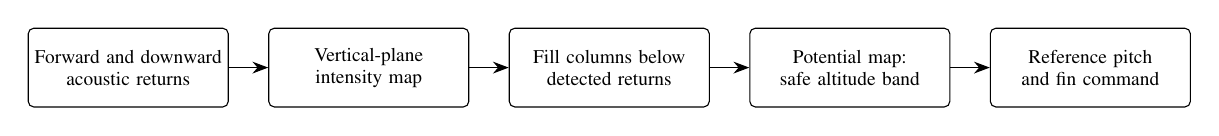
\begin{tikzpicture}[
  >={Stealth[length=2mm]},
  box/.style={draw, rounded corners=2pt, align=center, text width=24mm, minimum height=10mm, font=\scriptsize, inner sep=2pt},
  node distance=5mm and 5mm]
  \node[box] (a) {Forward and downward\\acoustic returns};
  \node[box, right=of a] (b) {Vertical-plane\\intensity map};
  \node[box, right=of b] (c) {Fill columns below\\detected returns};
  \node[box, right=of c] (d) {Potential map:\\safe altitude band};
  \node[box, right=of d] (e) {Reference pitch\\and fin command};
  \draw[->] (a) -- (b);
  \draw[->] (b) -- (c);
  \draw[->] (c) -- (d);
  \draw[->] (d) -- (e);
\end{tikzpicture}
\caption{Terrain-tracking pipeline: raw returns become a single pitch command. Adapted from \textcite{maki}.}
\label{fig:pipeline}
\end{figure}
 
The GODZILA-based system of \textcite{godzila} reaches a comparable outcome by a different route. It solves an optimisation cost function per measurement, penalising deviation from the target direction, motion toward detected obstacles, and backtracking into visited coordinates. For near-seafloor operation it applies depth-modulated directional weighting, tighter vertically than horizontally, so the vehicle reacts aggressively to seabed rises while still hugging the bottom. Acting only on current measurements makes it robust to the navigation drift that characterises towed systems. Both methods therefore produce a vertical command from immediate sensor data without an accurate global position estimate, which is the sensing regime a towed rig operates in.
 
Both sources also identify a persistent trade-off between computing power and endurance, where the processing needed for complex sonar interpretation adds mass and volume that degrade stability \parencite{kot2024,godzila}. Almost all of this work assumes omnidirectional propulsion, and the shortage of high-quality underwater datasets remains a bottleneck for applying learned methods to tasks such as coastal pest detection \parencite{kot2022,cao}.
 
% ============================================================
\subsection{Modular Design, Materials and Enclosures}
% ============================================================
\label{modular_lit}
Modularity is the least-studied part of this design space: the towed-camera literature treats platforms as single units, so guidance comes from marine materials practice and distributed embedded systems rather than from comparable vehicles.
 
Non-critical structure such as wings and fairings can be printed in ASA, PETG, or ABS, which offers better UV resistance, strength and water resilience than PLA \parencite{asa}. Electronics housings need a different standard: sealed enclosures with greased O-rings, whose service life is governed by seal maintenance rather than by housing material \parencite{orings}, with marine-grade plastics and aluminium. Treating the printed shell itself as the pressure boundary would remove the need for internal enclosures. Still, fused-deposition parts are porous along layer boundaries and a resin coating creates a single failure surface whose breach floods the system. In contrast, several small sealed enclosures cost one module per seal failure. A sealed strong material tube near the leading edge can both house critical components and carry load between modules.
 
Coordinating fin actuators across units needs a defined master--slave relationship, because a module outboard of the master must drive both of its surfaces in the same sense so the array behaves as one continuous foil. The ESP32 supports I\textsuperscript{2}C master--slave operation between units \parencite{esp32} and combines adequate processing for a PID loop with small size and low power draw, suiting an architecture where each slave reads its own sensors and reports to a master that returns actuator commands. Inter-module connections require purpose-built watertight connectors \parencite{connectors}, and potting resists water, pressure and corrosion at the cost of maintenance access and heat dissipation.
 
No reviewed towed-camera study addresses multi-unit coordination. Synchronising control surfaces across physically coupled bodies sharing a single tow point, where one module's lift alters its neighbours' trim, has no direct precedent in the marine survey literature.
 
% ============================================================
\subsection{Evaluation Approaches}
% ============================================================
\label{lit_eval}
Published work evaluates towed camera systems against two standards: controlled-environment repeatability and field comparison against an existing method.
 
Tank or pool testing removes current, waves, and visibility as testing variables so repeated runs can be attributed to the control system. Although pool depth and length limit the available tow speed and duration, results characterise controller behaviour rather than survey performance. Field comparison is how the published work establishes value: \textcite{cresswell} benchmark against diver transects on the same reef, \textcite{sheehan} compare platform classes across the same habitats on imagery quality, seabed impact and current tolerance, and \textcite{lembke_cbass} report time-in-band altitude statistics, the most transferable metric because it is directly comparable across platforms. The metrics that follow are altitude error distribution and time-in-band, pitch and roll stability, drag coefficient at survey speed, and obstacle clearance success rate, measured against the same rig with fins fixed so that active control is isolated from hull geometry.
 
% ============================================================
\section{Research Gaps}
% ============================================================
\label{research_gaps}
The literature gives a strong foundation in towed platform dynamics, acoustic sensing and avoidance planning, but still, gaps sit across this project's path.
 
\begin{enumerate}[leftmargin=*, itemsep=2pt]
  \item Obstacle avoidance has not been adapted to cable-constrained platforms. Methods such as those of \textcite{maki} and \textcite{godzila} assume a self-propelled vessel with omnidirectional authority. A towed body cannot command lateral motion, cannot stop, and has vertical authority bounded by control-surface lift and cable tension. Whether these methods still perform when the command space is reduced to one rate-limited axis is untested.
  \item The low-cost end of the flying tow platform class is underrepresented. Non-contact systems are either commercial products with undisclosed internals \parencite{seavu} or research platforms built to research budgets \parencite{controllable2005,dynamics2000,hydrofoil}. Whether adequate altitude holding is achievable with hobby-grade servos, ultrasonic ranging and a microcontroller determines whether the approach is deployable by a small dive operator.
\end{enumerate}
 
% ============================================================
\section{Research Questions}
% ============================================================
\label{research_questions}
Each question below maps to a gap above and to a measurable outcome.
 \begin{table}[htbp]
\centering
\footnotesize
\setlength{\tabcolsep}{4pt}
\renewcommand{\arraystretch}{1.15}
\caption{Research questions, the gaps they address, how each is measured and the expected outcome.}
\label{tab:research_questions}
\begin{tabularx}{\textwidth}{@{}>{\centering\arraybackslash}p{4mm}
                              >{\raggedright\arraybackslash}X
                              >{\centering\arraybackslash}p{8mm}
                              >{\raggedright\arraybackslash}X
                              >{\raggedright\arraybackslash}X@{}}
\toprule
\textbf{\#} & \textbf{Question} & \textbf{Gap} & \textbf{Measured by} & \textbf{Hypothesis} \\
\midrule
1 & Can active fin control improve altitude stability over a passive tow baseline at survey speed?
  & 2
  & Altitude error distribution and time within the 0.5--1.5\,m band about the 1\,m target, against the same rig with fins fixed
  & Yes: active fin control will have less rolling and stay in the 0.5--1.5\,m band for longer than passive. Changing depth will always require active fin control. \\
\addlinespace
2 & Can forward-facing acoustic sensing keep a towed rig clear of obstacles while holding an altitude low enough for Caulerpa imaging?
  & 1
  & Clearance success rate over a terrain course, and altitude held during and after each avoidance event
  & Yes: previous literature has shown that sensors can detect obstacles with significant room for avoidance. \\
\addlinespace
3 & Can a foil design perform the required manoeuvres by harnessing tension from an angled tow rope?
  & 2
  & Required pitch rate versus achievable pitch rate across obstacle profiles
  & Yes: control surfaces redirect the flow the tow already supplies into vertical force at negligible power cost (Section~\ref{depth_lit}), so this design should act similarly \\
\bottomrule
\end{tabularx}
\end{table}
 
Question 1 is the primary one. If active control does not beat a passive baseline, the added complexity is unjustified.
 
\section{Methods}
This section first sets out the design requirements and constraints from the problem specification, then describes the design and how it was validated and tested.
% Intro between each section and subsection
\subsection{Design Breakdown}
\label{design_specs}
The design specifications for the tow camera were:
\begin{itemize}
    \item Low towing speed: operate at a steady towing speed of 0.5--1.0\,m/s, nominally $1\,\mathrm{m/s}$, which keeps camera footage sharp and gives the detection system enough time to identify Caulerpa.
    \item Survey altitude: hold a 1\,m target altitude within the 0.5--1.5\,m band for longer than the 60--80\% time-in-band reported for a passive towed platform \parencite{lembke_cbass} (Section~\ref{tow_class}).
    \item Obstacle avoidance: detect a 0.3\,m seabed rise at least 2.5\,m ahead and pitch up to a $20^\circ$ climb within about 1\,s, a pitch rate of at least $20^\circ$/s, so the rig clears it at 1\,m/s (Equation~\eqref{eq:horizon}).
    \item Camera payload: carry an underwater camera that provides images suitable for automated Caulerpa detection.
    \item Parallel operation: allow several units to be towed, so a larger area of seabed can be surveyed in a single pass.
\end{itemize}

The design constraints were:
\begin{itemize}
    \item Size: the unit must be small and light enough to be carried by hand and to fit into regular transportation, such as the boot of a car or a small boat cabin.
    \item Cost and manufacturing: the unit must be low cost and use manufacturing methods such as 3D printing, so that production can be scaled.
\end{itemize}
 
\subsection{Foil Selection and Force Balance}
\label{force_balance}
To meet the design specification of a low towing speed, the system uses a NACA 5518 foil section (5\% maximum camber at 50\% chord, 18\% thickness-to-chord ratio) mounted in an inverted configuration, so that the section generates down force directly and can keep the tension from the tow cable. A symmetric foil produces zero lift at zero angle of attack and must be run at a comparatively large negative control effort to generate the required down force, creating additional drag. A cambered section produces a non-zero force at zero geometric incidence, $\alpha_{L0}$.

Evaluated for the NACA 5518 camber line, thin-aerofoil theory places $\alpha_{L0}$ in the region of $-5^\circ$ to $-6^\circ$, consistent with published data for comparable 4-digit sections \parencite{abbott1959}. 

The resulting downward force is:
\begin{equation}
L = \tfrac{1}{2}\rho V^2 S \, C_L
\end{equation}
where $\rho = 1025\ \text{kg/m}^3$ (seawater), $V$ is towing speed, and $S$ is planform area. At the design towing speed of 0.5 to 1.0 m/s, dynamic pressure $\tfrac{1}{2}\rho V^2$ ranges from 128 to 513 Pa. Foil sizing is detailed in the co-worker's companion report \parencite{chittenden2026}.

Taking moments about the CoM, with nose-up positive, steady trim requires
\begin{equation}
L\,d_L + T\,d_T + D\,d_D + B\,d_B = 0,
\label{eq:moment}
\end{equation}
where each $d$ is a signed perpendicular moment arm, defined so that a positive force-arm product produces a nose-up moment. Weight acts through the CoM and therefore contributes no moment about it. Buoyancy acts through the centre of buoyancy and can contribute a restoring moment when the rig pitches. Its contribution can be neglected only where its line of action passes through the CoM or its moment is demonstrably small. Fin deflection changes the hydrodynamic forces and their moments, allowing the controller to adjust pitch and hence the rig's vertical trajectory (Section~\ref{sec:activeStab}).
 
\subsection{Tow Attachment Point Geometry}
\label{tow_attach}
The tow attachment is located on the upper surface of the body. Its pitching effect depends on both its horizontal and vertical position relative to the CoM and on the rope angle. In side-view coordinates, with $x_T$ measured horizontally forward and $z_T$ vertically upward from the CoM, the nose-up moment from tension is $M_T = T(x_T\sin\gamma - z_T\cos\gamma)$, where $\gamma$ is the rope's elevation above horizontal. The upward tension component can produce a nose-up moment at a forward attachment, while the forward component produces a nose-down moment at an elevated attachment.

An attachment directly above the CoM therefore does not generally eliminate the rope moment. Zero moment occurs when the line of action of tension passes through the CoM. Because the rope angle changes with towing geometry and rig position, an attachment that gives little moment under one condition may require substantial fin correction under another. The design objective is to reduce the steady pitching bias at the intended operating condition while retaining enough control authority for climbing and descending.

During water entry, the forward component of tension acting above the CoM can encourage a nose-down response. The submerged trim must then be assessed using the complete force and moment balance. The spar substitution described in Section~\ref{construct} moved the CoM forward, changing the attachment offsets. The end-cap redesign in Experiment Four moved the attachment forward to reduce the nose-down bias observed in Experiment Three; the remaining trim requirement was subsequently assessed from the logged fin response.
 
\begin{figure}[ht]
\centering
\includegraphics[width=0.34\textwidth]{Figures/P4p_CoM}
\caption{Internal CAD layout showing structural openings and CoM-relevant component placement.}
\end{figure}
 
\subsection{Construction}
\label{construct}
With the constraints of scalability and manufacturing, the body is predominantly 3D printed for the ease of location and repeatability. The material used is PETG for its UV resistance and water resistance relative to PLA. The leading-edge spar, originally a hollow aluminium tube providing both the primary load path and the mechanical interface between printed sections, was replaced late in fabrication with a solid stainless steel threaded rod for the full-scale prototype. This substitution materially altered the mass distribution and is the direct cause of the attachment-point result reported in Section \ref{sec:Exp2}. The ends of the steel rod were tightened with nuts during the experiment, however, in the commercial model, these rods will be cut short so they do not protrude from the sides as they did in the experiments (Appendix~\ref{sec:AppCompendium}).

Figure~\ref{fig:CadExploded} shows the full exploded view of the final model. Each section is individually 3D-printed and can be replaced for repairs. This was decided for the design constraint of low cost and ease of manufacturing.  The figure clearly shows the control fins and the gears used for active control (Section~\ref{sec:activeStab}), and the final connection point chosen (the foremost hole on the end cap). The hole in the main body is where the camera is held. 

\begin{figure} [ht]
    \centering
    \includegraphics[width=0.5\linewidth]{Figures/Exploded View P4p.png}
    \caption{Exploded view of the design.}
    \label{fig:CadExploded}
\end{figure}

From end cap to end cap, the rig is 800\, mm, and 300\, mm from the leading edge to the end of the tail. This satisfies the specification of being small enough for transport, as well as all pieces being small enough for commercially available 3D printers. 
\subsection{Sensor}
\label{tow_sensors}
The sensor suite comprises eight ultrasonic transducers (four pairs), an IMU (BNO085, 9-DOF with onboard sensor fusion), and an optical camera, mounted directly to the 3D printed end caps. Altitude from time-of-flight is $h = ct/2$, with $c \approx 1500\ \text{m/s}$ in seawater; at the 0.5 - 1.0 m target altitude, expected round-trip time is 0.67 - 1.33 ms.

Overhang detection uses the conservative highest-point rule. For a forward sensor at a given range and elevation, the minimum across all forward sensors is taken as the binding constraint, detects the highest point, and plus the threshold altitude. Sensors can detect points at their different angles using the cosine of the IMU and the mounting angle, in combination with the distance value. 

Depth of the system is treated as the angle-adjusted distance of the different ultrasonic sensors (adjusted to the cos of the mounting angles). Due to the uneven terrain of the seafloor, the altitude sensors will read different values, so the measured altitude will be the minimum value. This is a safety feature so it is always far away from the seabed to avoid scrapes, the alternative of using the mean of the two values could cause sharp cliffs between the sensors to be treated as flat terrain at the mid-height. 

The optical sensor sits in a sealed length of plastic pipe, closed by a custom threaded end cap carrying a flush optical window sealed with O-rings under compression, a standard face-seal arrangement. The cap is printed in PETG, but PETG's inter-layer micro-porosity is a leak risk, mitigated by a reduced print speed (letting each layer consolidate) and an exterior waterproofing spray coat that bridges surface pores without touching the seal faces or window.
 
\subsection{Stability and Power System}
\label{power_system}
As this requires active control, a power system is required. This needs to be safely designed to meet waterproofing restrictions, as well as meet the design constraints of size and cost, while also being powerful enough to meet the specifications of avoidance. 
\subsection{Passive and Active Stability}
\label{sec:activeStab}
Bilateral symmetry removes steady-state yaw bias, and a CoM held below the centre of buoyancy gives a passive righting moment in roll, reducing active control to the single pitch/depth axis.

The first controller was a closed discrete PID loop on the master ESP32 (20 Hz) with anti-windup clamping the control when $\delta_f$ saturates at its $\pm25^\circ$ mechanical limit. It commanded pitch based on the altitude error, however, this controller failed in Experiment Five (Section~\ref{sec:Exp5}). It was then switched for a cascaded PI controller relating altitude to pitch, then a P controller commanding the fins from pitch error. A Kalman filter was also used to estimate altitude by combining the noisy measurements from the IMU and ultrasonic sensors. 
 
\subsection{Power Architecture}
 
\begin{figure}[ht]
\centering
\begin{minipage}{0.44\textwidth}
\centering
\includegraphics[width=\linewidth]{Figures/P4p_Power_Diagram.png}
\caption{System power and data architecture.}
\end{minipage}
\hfill
\begin{minipage}{0.5\textwidth}
\centering
\includegraphics[width=\linewidth]{Figures/P4p_Elec_Schem.png}
\caption{Wiring schematic.}
\label{fig:ElectScheme}
\end{minipage}
\end{figure}


 
Power and data share a single PoE tether down the tow cable rather than separate cores, consistent with the modular, low-drag cabling goal. On the camera side, a PoE splitter separates the 12 V rail, feeding a battery management system (BMS) that charges a 4S LiPo pack (14.8 V nominal), from the Ethernet data path, which feeds the switch, camera, and (via an Ethernet-to-SPI module) the master ESP32. This is deliberate: PoE alone cannot supply the system's peak load. Each servo is rated up to 9 A at 8.4 V (75.6 W) under stall, though sustained draw is under 20 W per servo; two servos can therefore demand well over 100 W momentarily against a continuous budget of roughly 50 W (Table 1). Local battery buffering decouples this peak from the tether, which need only sustain the pack's average charge balance. 

Two buck converters step the 14.8 V bus down to a 5 V logic rail (90\% efficiency) and a 7.4 V/8.4 V servo rail (capacitor-smoothed). The master ESP32 bridges an Ethernet module by SPI, a UART/RS-485 expander to the sensor array and IMU, and PWM to both servos; since the array runs 5 V logic against the ESP32's 3.3 V GPIOs, level-shifting on the RS-485 lines is required and flagged as an open risk item.
 
\begin{table}[ht]
\centering
\small
\begin{tabular}{lll}
\toprule
\textbf{Component} & \textbf{Rail} & \textbf{Draw} \\
\midrule
Camera & 5 V (Ethernet-side) & $\leq$1.5 W \\
ESP32 logic & 3.3 V (reg.\ from 5 V) & $\sim$1 W cont., 2.5 W peak \\
Ultrasonic array ($\times$8) & 5 V & 0.8 W (0.16 A) \\
Filtering capacitors & 5 V rail & $\leq$0.3 W quiescent \\
Servo (each) & 7.4-8.4 V & $<$20 W cont.; 51.8 - 75.6 W stall \\
\midrule
System continuous total & --- & $\approx$50 W (incl.\ 90\% buck eff.) \\
\bottomrule
\end{tabular}
\caption{Power budget by component, from the system power diagram.}
\end{table}

\section{Test Programme}
\label{sec:planner}

\subsection{Common Procedure}
\label{sec:procedure}
All full-scale trials were run in the University of Auckland pool, which is 2\,m deep. The rig was attached by carabiners at both end caps to a braided rope forming a symmetric V-bridle, and was pulled by hand from the far end of the pool. The rope was 20\,m long, but the effective rope was 1.5\, m, as it was held at the surface $\approx$ 1\, m ahead of the rig to avoid scraping along the pool floor. Tow speed was estimated from each video by timing the rig between pool lane markings of known spacing. Each configuration was run 3 times. From Experiment Four onward, the firmware logged all eight ultrasonic ranges with validity flags, roll, pitch and yaw, current and target altitude, and both fin angles to CSV at 10\,Hz (Appendix~\ref{sec:AppCSV}). Videos and logs are listed in the research compendium (Appendix~\ref{sec:AppCompendium}).

\subsection{Experimental Programme}
Table~\ref{tab:testplan} links each experiment to the research questions.

\begin{table}[ht]
\centering
\footnotesize
\caption{Experimental programme and its link to the research questions.}
\label{tab:testplan}
\begin{tabular}{@{}>{\raggedright\arraybackslash}p{10mm}>{\raggedright\arraybackslash}p{44mm}>{\centering\arraybackslash}p{10mm}>{\raggedright\arraybackslash}p{38mm}>{\raggedright\arraybackslash}p{32mm}@{}}
\toprule
\textbf{Exp.} & \textbf{Purpose} & \textbf{RQ} & \textbf{Data recorded} & \textbf{Outcome} \\
\midrule
1 & Validate passive diving at 1/7th scale (Froude-matched) & 1 & Video, qualitative trim & Concept confirmed \\
2 & Full-scale passive behaviour, fins locked & 1 & Video, qualitative trim & Roll unstable; enclosure leaked \\
3 & Select tow point with simple roll and altitude control & 1, 3 & Video, qualitative trim & Nose-down bias at all points; end caps redesigned \\
4 & Verify sensing, logging and vertical response & 1, 2 & CSV log & Sensing and actuation confirmed \\
5 & First closed-loop altitude control (single-loop PID) & 1 & CSV log & Sustained oscillation \\
Sim. & Identify model and redesign controller & 1, 2, 3 & Simulated states & Cascaded PI--P selected \\
6 & Cascaded control against fins-fixed baseline; set-point step; obstacle & 1, 2, 3 & CSV log, video, camera frames & Successful Towing\\
\bottomrule
\end{tabular}
\end{table}
Videos of all experiments are available in \ref{sec:AppCompendium}.
\section{Experiment One: Scale Model}
\label{sec:Exp1}

The first experiment used a 1/7th-scale model to assess whether the proposed foil and tow-point arrangement produced a passive diving response before full-scale fabrication. A single physical model cannot match both the Reynolds number $Re = VL/\nu$ and the Froude number $Fr = V/\sqrt{gL}$ of the full-scale system. The aspect of interest here is the diving moment produced by tow tension acting about the CoM against buoyancy, which is governed by gravity and buoyancy rather than viscous shear, so the Froude number was matched. This requires the model speed to scale as $V_m = V_f\sqrt{L_m/L_f}$. At a length ratio of 1/7, $V_m \approx 0.378\,V_f$, so the 1\,m/s design speed corresponds to a model speed of 0.38\,m/s. The model was towed at approximately 0.2\,m/s over 3 runs, which corresponds to $V_f = 0.2\sqrt{7} \approx 0.53$\,m/s at full scale, at the lower end of the intended 0.5--1.0\,m/s operating range.

This speed correspondence alone does not establish full dynamic similarity. Reynolds number was not matched, and geometric scaling does not by itself ensure equivalent mass distribution, buoyancy or towing geometry. The experiment was therefore interpreted as a qualitative assessment of diving behaviour. The observed nose-down response and submerged towing supported proceeding to full-scale fabrication, while quantitative lift, drag, trim and stability performance required full-scale testing.

The model carried a longitudinal tail fin on the centreline for passive yaw stability. A single tow point was placed on the upper surface above the estimated CoM, and no sensors or electronics were fitted. This isolates the hydrodynamic behaviour of the hull from the effect of electronics mass on trim, so a failure to dive could be attributed to the hull geometry rather than to a mass-distribution error. The video is listed in Appendix~\ref{sec:AppCompendium}.
 
\begin{figure}[ht]
\centering
\includegraphics[width=0.32\textwidth]{Figures/P4p Prototpe Pool.png}
\caption{1/7th-scale model under tow, diving from a single central attachment point.}
\label{fig:Exp1}
\end{figure}
 
\subsection{Results}
When tension was applied, the model pitched nose-down, as predicted for an attachment on the upper surface, settled at a stable negative incidence, and dived below the surface (Figure~\ref{fig:Exp1}). No divergent pitch or yaw oscillation was observed in any of the 3 runs, and the tail fin held the heading aligned with the tow direction. These results confirmed the downforce mechanism and justified full-scale fabrication. Drag and stability margins depend on Reynolds number and were left to be checked at full scale.
 
\subsection{Implications for Full-Scale Design}
The inverted cambered foil and the tow point above the CoM were carried forward unchanged, since the model showed the correct sign and stability of the diving response.

The model showed that the hull is directionally stable when it carries vertical fin area; it did not test the hull without a fin. The full-scale design therefore keeps vertical fin area, but moves it from the centreline to plates on the two end caps. This keeps the centreline clear for the electronics and camera housings, adds roll damping at the span tips, and integrates the fins with the end caps that already carry the sensors, reducing part count and stowed size. Yaw behaviour of this arrangement is assessed in the full-scale trials.
 
\section{Experiment Two: Full-Scale Passive Behaviour}
\label{sec:Exp2}

The full-scale prototype replaced the model's single central attachment with two attachment points at the end caps, for two reasons. First, the end caps already carry the ultrasonic hardware and the structural interface to the leading-edge spar, so attaching the tow there avoids a separate central fitting and its mass and drag. Second, two attachments give load redundancy: if one fails, the rig remains connected. With two attachments, the rope forms a V-bridle, and for equal leg lengths the effective tow point lies midway between the end-cap attachments.
 
\subsection{Setup}
The procedure of Section~\ref{sec:procedure} was used, at an estimated 1\,m/s. No electronics were powered. The servos were locked at their trim position, and the servo leads ran into a temporary plastic container standing in for the electronics enclosure. The end cap and fixed wing provide four attachment holes (fore, mid-fore, mid-aft and aft), so the effective tow point can be moved chordwise without new hardware. A pre-trial CAD mass analysis placed the CoM near mid-chord, so the middle hole was used. Immediately before the trial, the aluminium spar was replaced with the stainless-steel rod (Section~\ref{construct}), which moved the CoM forward.
 
\begin{figure}[ht]
\centering
\begin{minipage}{0.44\textwidth}
\centering
\includegraphics[width=\textwidth]{Figures/P4p Prototype full size.jpg}
\caption{Prototype with dual end-cap attachment points visible.}
\label{fig:proto}
\end{minipage}
\hfill
\begin{minipage}{0.44\textwidth}
\centering
\includegraphics[width=\textwidth]{Figures/P4p Prototype Swimming.png}
\caption{Prototype under tow.}
\label{fig:protoTow}
\end{minipage}
\end{figure}
 
\subsection{Results}
The rig dived under tow but was unstable in roll (Figure~\ref{fig:protoTow}). During the runs the temporary container began to float out of the electronics bay and took on water.

These results cannot serve as the passive baseline for Research Question 1. The roll instability may come from the hull, from the buoyant, flooding container shifting the centres of mass and buoyancy, or from fins that were not locked exactly at trim, and this experiment cannot separate those causes. The fins-fixed baseline is therefore measured in Experiment Six with the final enclosure and full logging. The experiment did show that the enclosure must be rigid, sealed and secured, and that the tow point needed re-selecting after the spar change.

\section{Experiment Three: Tow Point Selection}
\label{sec:Exp3}

Experiment Three repeated the setup of Experiment Two with the electronics in a sealed PVC pipe and simple roll and altitude control active, and compared the forward, middle and aft attachment holes.

\subsection{Results}
Table~\ref{tab:attach} summarises the observed behaviour. The forward hole gave consistent pitch with little fin correction, while the middle and aft holes produced a persistent nose-down bias that increased drag. However, even at the forward hole the rig could not pitch up enough to climb.

\begin{table}[ht]
\centering
\caption{Pool trial outcome by attachment point.}
\label{tab:attach}
\begin{tabular}{lll}
\toprule
\textbf{Attachment point} & \textbf{Observed behaviour} \\
\midrule
Forward (selected) & Consistent pitch; could not pitch up to climb\\
Middle & Moderate nose-down bias \\
Aft & Large nose-down bias \\
\bottomrule
\end{tabular}
\end{table}

Equation~\eqref{eq:moment} explains this pattern. After the spar change the CoM lay forward of all three holes, so the upward component of rope tension acted behind the CoM at every hole and produced a nose-down moment whose arm, and therefore size, grew from forward to aft. At the forward hole the moment was smallest, which gave the steadiest trim, but it remained nose-down, and the fins could not overcome it to pitch the rig up. To meet the vertical-movement specification the attachment had to move forward until it again sat above the CoM, which required new end caps.

\section{Experiment Four: Sensing and Vertical Response}
\label{sec:Exp4}

The end caps were redesigned with the attachment moved forward to sit above the shifted CoM, and with large side plates that act as the passive yaw fins. To keep the rig transportable, the plates were limited to approximately $300 \times 60$\,mm. The ultrasonic wires feed through a small slot in each end cap, and each transducer is clamped into its own seat (Figure~\ref{fig:EndCap}). The wires are soldered directly to the electronics because waterproof connectors are expensive and difficult to disconnect and reconnect, which serves the cost and manufacturing constraints. The transducers were mounted at $-10^\circ$, $+10^\circ$, $+35^\circ$ and $90^\circ$ from vertical (Section~\ref{tow_sensors}), so that at least one beam points close to vertical over the full pitch range and the remaining beams look ahead for obstacles.

\begin{figure}[ht]
    \centering
    \includegraphics[width=0.5\linewidth]{Figures/End Cap Image P4p.png}
    \caption{Redesigned end cap with the forward attachment, yaw plate and transducer seats.}
    \label{fig:EndCap}
\end{figure}

\begin{figure}[ht]
\centering
\begin{minipage}{0.44\textwidth}
\centering
\includegraphics[width=\textwidth]{Figures/P4p Lab Full.jpg}
\caption{Redesigned rig in the lab.}
\label{fig:labFull}
\end{minipage}
\hfill
\begin{minipage}{0.44\textwidth}
\centering
\includegraphics[width=\textwidth]{Figures/P4p Sensor Mount.jpg}
\caption{Transducer placement on the end cap.}
\label{fig:sensorMount}
\end{minipage}
\end{figure}

\subsection{Purpose and Setup}
This experiment verified that the full sensor suite could be read and logged during a tow, and that the rig moves vertically in response to fin commands. The procedure of Section~\ref{sec:procedure} was used with the servos powered and all eight transducers and the IMU logging. The controller used uncorrected ranges, without compensation for mounting angle or pitch, so altitude holding was not expected in this experiment. Two runs were logged at an estimated 1\,m/s.

\subsection{Results}
Figure~\ref{fig:Test1Results} shows the ranges from the first run. The forward ($90^\circ$) beams, shown separately in the legend, measure the distance to the pool wall ahead rather than altitude.

\begin{figure}[ht]
    \centering
    \includegraphics[width=0.8\linewidth]{Figures/Drive_By_Results.png}
    \caption{Experiment Four, run 1: range from each of the eight transducers against time. Forward ($90^\circ$) beams measure distance to the pool wall; the remaining beams measure distance to the floor.}
    \label{fig:Test1Results}
\end{figure}

\begin{figure}[ht]
    \centering
    \includegraphics[width=0.8\linewidth]{Figures/Fin_Down_Results.png}
    \caption{Experiment Four, run 2 (fins commanded down): range from each transducer over time.}
    \label{fig:Test2Results}
\end{figure}

\begin{figure}[ht]
    \centering
    \includegraphics[width=0.8\linewidth]{Figures/Fin_Down_Constrained.png}
    \caption{Experiment Four, run 2: downward-beam ranges with the axis limited to the pool depth.}
    \label{fig:Test2Axis}
\end{figure}

The IMU reads $-80^\circ$ when the rig is level, so Figure~\ref{fig:Test2Pitch} plots pitch relative to level (logged value $+80^\circ$). The rig floated at the surface until tension was applied at about 30\,s, pitched nose-down, reached its target altitude by about 40\,s, and levelled out.

\begin{figure}[ht]
    \centering
    \includegraphics[width=0.8\linewidth]{Figures/sensor_pitch.png}
    \caption{Experiment Four, run 2: pitch relative to level against time, on the same time axis as Figure~\ref{fig:Test2Results}.}
    \label{fig:Test2Pitch}
\end{figure}

Between 30 and 50\,s and between 75 and 90\,s, changes in downward range coincide with departures of pitch from level (Figures~\ref{fig:Test2Results} and~\ref{fig:Test2Pitch}). These records are consistent with changes in the rig's attitude and vertical trajectory, but uncorrected slant range cannot distinguish the two effects. Pitch changes the beam direction even when the rig's altitude remains constant, so correlation between raw range and pitch is not independent evidence of vertical displacement.

The logs demonstrate acquisition of ultrasonic and IMU data during towing. Qualitative vertical movement showed rapid switching between trim and diving (Appendix~\ref{sec:AppCompendium}). The logged run (\texttt{Exp4.csv}, 379 samples over 37.8\,s at 10\,Hz) quantifies the dropout: the altitude estimate was valid in 84\% of samples, but individual transducers returned a valid echo in only 7--55\% of samples, so most samples relied on one or two beams. This motivated the beam selection and stale-value handling of Section~\ref{sec:kalman}. Quantitative altitude-holding performance is evaluated in the later experiments using angle compensation and an explicitly stated measurement method. Experiment Four therefore established the sensing and logging capability needed for those tests rather than demonstrating accurate altitude control.

\section{Experiment Five: Single-Loop PID Control}
\label{sec:Exp5}

Experiment Five was the first closed-loop altitude test. Ranges were corrected for mounting angle and measured pitch, and the single-loop PID of Section~\ref{sec:activeStab} set the fin angle from altitude error. When above the target, it commanded the fins to pitch the rig down, and below the target to pitch it up. The free rope was lengthened to 3\,m, compared with 1.5\,m in Experiment Four, to test whether the controller could hold altitude without a short, steep rope constraining the rig.

Two implementation faults were found during testing. First, the firmware discarded the previous range before a new one was available, which made the fins jitter; it was changed to retain the most recent valid reading. Second, when the rig pitched steeply, the downward beams lost the floor because the reflected signal no longer returned to the transducer.

\subsection{Results}
The rig dived, detected the pool floor and pitched up in response, but it did not settle. As the rig reached the target the fins returned to trim while the body kept its pitch, so it passed through the target and the cycle repeated in the opposite direction. The logged run (\texttt{Exp5.csv}) used a 500\,mm target (Figure~\ref{fig:Exp5}). Over the 18\,s towed section, the altitude estimate reached minima of 435\,mm and 614\,mm at the ends of two descents 8.9\,s apart, and the fins sat at the nose-down limit for 1.0\,s and 2.6\,s during those descents. Only 22\% of valid altitude samples lay within $\pm250$\,mm of the target, and 12\% within $\pm100$\,mm. This is well below the 60--80\% of time in the ideal altitude band that \textcite{lembke_cbass} report for a passive towed platform, although their band was set for a deeper survey. In addition, 48 of the 160 valid samples exceeded the 2\,m pool depth, reaching 5.34\,m. These were echoes from beyond the floor that the firmware accepted because it applied no upper range limit. When the beams lost the floor, the controller kept acting on the last valid reading: the estimate held 435\,mm and 614\,mm for about 0.9\,s each, which increased the overshoot. Section~\ref{sec:cascade} examines the dynamics underlying the observed oscillation and explains the motivation for the cascaded redesign.

\begin{figure}
    \centering
    \includegraphics[width=0.5\linewidth]{Figures/Exp5_height_vs_target.png}
    \caption{Experiment Five: estimated altitude against the 500\,mm target.}
    \label{fig:Exp5}
\end{figure}

Steady altitude was not achieved, but the experiment showed that the rig now responds actively to its altitude above the pool floor rather than relying on a steep rope angle for stability. The logged pitch and fin data from this experiment (\texttt{sensor-\allowbreak log-\allowbreak goodRunPopedatAPoint.csv}) were used to identify the pitch model in Section~\ref{sec:sim_model}.
\section{Simulation and Controller Redesign}
\label{sec:sim}

Experiment Five exposed two problems: altitude feedback became stale when the downward beams lost the floor, and the single-loop controller did not settle at the target. A software-in-the-loop simulation was developed to tune the estimator and controller while the rig was unavailable. The simulator compiles the firmware control implementation directly, replacing the hardware interfaces with simulated sonar, IMU and servo responses. This allows the control logic to be exercised against known states before pool testing. The controller operates at 50\,Hz, while the body model is integrated in 1\,ms steps.

\subsection{Plant and Sensor Models}
\label{sec:sim_model}

Two alternative body models are implemented. The generic model represents pitch as a damped second-order response to fin deflection:
\begin{equation}
\ddot\theta = \omega_n^2(k_f\delta-\theta)
 - 2\zeta\omega_n\dot\theta,
\qquad
\omega_n = 2\frac{U}{U_{\mathrm{ref}}}\ \mathrm{rad/s},
\end{equation}
where $k_f=1$, $\zeta=0.7$ and $U_{\mathrm{ref}}=1$\,m/s. A flight-path angle $\gamma_f$ follows pitch with a 0.3\,s time constant, and determines the vertical velocity:
\begin{equation}
\dot\gamma_f = \frac{\theta-\gamma_f}{0.3\ \mathrm{s}},
\qquad
\dot z = U\sin\gamma_f.
\end{equation}

The towed-foil model couples an empirical pitch response to a vertical force balance. Its implemented pitch equation is
\begin{equation}
\dot\theta = k_\delta\delta
 - \frac{\theta-\theta_r}{\tau_r},
\qquad
\theta_r = \tan^{-1}\!\left(\frac{H_T-h}{X_T}\right),
\label{eq:tow_pitch}
\end{equation}
where $h$ is clearance above the local seabed, $H_T=3$\,m and $X_T=7$\,m are nominal tow-point offsets, $k_\delta=0.52\ \mathrm{(deg/s)/deg}$ and $\tau_r=1$\,s. Positive pitch is nose-up. The rope term pulls pitch towards the rope angle, so the pitching bias changes with altitude and attitude. The model does not apply a constant fitted pitch-rate offset or an explicit 0.3\,s transport delay.

The plotting script includes a routine for estimating fin-to-pitch-rate gain from a tow log. It fits $q_i\approx k_\delta f_i+c$ by duration-weighted least squares, using isolated data of when the rig was actually being towed rather than floating still, $|\phi|<20^\circ$, $|\theta|<45^\circ$, duration no greater than 1.2\,s and $|q_i|\leq40^\circ$/s. Fin commands are averaged over each interval shifted 0.3\,s earlier. When a fitted gain is supplied, it can replace $k_\delta$ in the tow scenario; the fitted intercept is not inserted into Equation~\eqref{eq:tow_pitch}. All results below use the simulator's default $k_\delta=0.52$, rather than claiming a new fit to experimental data.

In the towed-foil model, vertical motion follows
\begin{equation}
(m+m_a)\ddot z
 = L\cos\gamma_f-D\sin\gamma_f
 + F_{T,z}-(W-B),
\label{eq:sim_heave}
\end{equation}
with $\gamma_f=\tan^{-1}(\dot z/U)$. Lift and drag depend on relative flow speed and angle of attack $\alpha=\theta-\gamma_f$. The rope's upward force is approximated by
\begin{equation}
F_{T,z}=(D\cos\gamma_f+L\sin\gamma_f)\tan\theta_r.
\end{equation}
Here $L$ is signed lift, positive upward. The simulated foil has 0.25\,m chord, 0.60\,m span and inverted 5\% camber. Its lift curve uses a finite-aspect-ratio correction to thin-aerofoil theory, with an estimated stall limit and post-stall reduction. The mass is 8\,kg and equal buoyancy. Added mass is approximated by $m_a=\rho\pi c^2b/4$, using chord $c$ and span $b$. These are simplified force relationships and assumed parameters, not a validated six-degree-of-freedom hydrodynamic model.

The sensor model polls one of eight beams every 60\,ms, giving a 0.48\,s cycle. Each beam is ray-traced against the simulated seabed using its mounting angle and true pitch. Baseline runs use 12\,mm standard-deviation Gaussian range noise, a 20\% transaction-failure probability and a 5\,m maximum range. Near-field false echoes of 50-100\,mm can also be injected. The IMU model adds 0.2$^\circ$ attitude noise and 0.05\,m/s$^2$ vertical-acceleration noise, but does not replicate calibration error or long-term drift. Physical servo motion is limited to 350 servo-degrees/s, with six servo-degrees per degree of fin deflection.

This model has clear limitations. The closed-loop C++ simulation uses interpolated and delayed relationships derived from logged data ($k_\delta=0.52$) rather than fundamental equations of motion, so it may not capture behaviour outside the observed conditions. However, simplified models can still provide useful initial PI gains before physical testing is available. For example, \textcite{skogestad2003} presents PI tuning methods based on low-order models incorporating process gain and delay, supporting this model's use as a starting point for tuning, with subsequent experimental validation and refinement.


\subsection{Altitude Estimation}
\label{sec:kalman}

On each end cap, the firmware selects a fresh downward beam close to vertical after pitch compensation, with an 8$^\circ$ switching hysteresis. Each selected range is corrected for pitch and roll:
\begin{equation}
\label{beamheight}
h_i=r_i\cos(\beta_i+\theta)\cos\phi.
\end{equation}
The lower available end-cap value provides the conservative altitude measurement. A two-state Kalman filter estimates altitude and upward velocity \parencite{kalman1960}. It predicts between echoes using world-frame vertical acceleration when that input is valid, and assimilates each contributing sonar sample once. Sonar data become stale after 0.8\,s, the filter is reset when the last assimilated measurement is more than 1\,s old. Without valid altitude or attitude feedback, the controller commands a $+5^\circ$ fin offset as a climb fallback, whose physical effect still depends on available control authority.

The implemented filter has no innovation gate. Positive, geometrically usable false echoes can therefore enter the estimate, and the avoidance logic also acts directly on raw ranges.

For the baseline 60\,s towed-foil run described below, raw and filtered altitude were compared with simulation truth over the same available samples. The simulator writes controller estimates before advancing the body by one 20\,ms control period, but writes truth afterwards. Aligning each estimate with the preceding body state gives RMS errors of 11.11\,mm for raw sonar and 7.86\,mm for the Kalman estimate. These are estimation errors relative to the model state, distinct from altitude-tracking error relative to the target. They demonstrate noise reduction under the stated assumptions, rather than measured accuracy of the physical rig.

\subsection{Controller Redesign}
\label{sec:cascade}

Experiment Five showed that returning the fins towards trim as altitude error decreased did not necessarily remove the body's pitch or vertical motion. Slow sonar updates and stale measurements further complicated damping through altitude feedback alone. These observations motivated cascaded control, with an outer altitude PI loop and an inner pitch P loop \parencite{fossen2021} (Figure~\ref{fig:cascade}). They do not establish that every single-loop PID controller must fail.

Let $e=h_{\mathrm{sp}}-\hat h$, and let $I$ denote the integral contribution in pitch degrees. The main control relationships are
\begin{equation}
\theta_{\mathrm{ref}}=\operatorname{sat}_{\pm30^\circ}(K_p e_P+I),
\qquad
\delta_{\mathrm{cmd}}=\operatorname{sat}_{\pm25^\circ}
 \left[K_\theta(\theta_{\mathrm{ref}}-\theta)+\delta_{\mathrm{reflex}}\right],
\end{equation}
where $e_P=e$ outside the altitude deadband and is zero inside it. The deadband is entered at $|e|\leq15$\,mm and exited above 25\,mm. The integral is retained inside this band to support trim. Integration uses an error capped at $\pm100$\,mm and is paused when closing speed towards the target reaches 25\,mm/s, or when pitch or fin saturation would be driven further in the direction of the error. During avoidance or reflex action, integration may increase the climb command but cannot accumulate additional nose-down trim. The integral contribution is limited to $\pm30^\circ$ \parencite{astrom_hagglund2006}.

Both fins receive the same command; roll is used for range compensation rather than active roll control. Fin commands slew at 8$^\circ$/s normally and 24$^\circ$/s during emergency reflex action. With the rope angle held locally constant, substitution into Equation~\eqref{eq:tow_pitch} gives an ideal inner-loop time constant
\begin{equation}
\tau_{\mathrm{inner}}=
\frac{1}{k_\delta K_\theta+1/\tau_r}
\approx0.71\ \mathrm{s}
\end{equation}
for $K_\theta=0.8$. This local approximation excludes slew limits, changing rope geometry and heave coupling.

\begin{figure}[ht]
\centering
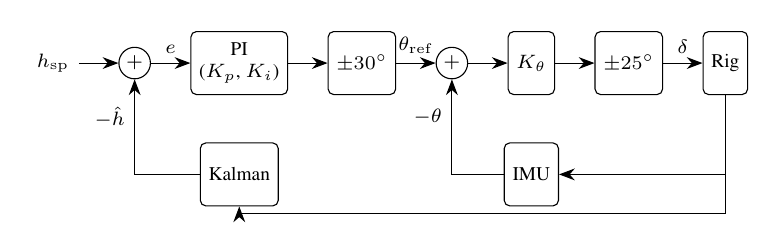
\begin{tikzpicture}[
  >={Stealth[length=2mm]},
  box/.style={draw, rounded corners=2pt, align=center, minimum height=8mm, font=\scriptsize, inner sep=3pt},
  sum/.style={draw, circle, inner sep=1.2pt, font=\scriptsize},
  node distance=4mm and 5mm]
  \node (sp) {\scriptsize $h_{\mathrm{sp}}$};
  \node[sum, right=of sp] (s1) {$+$};
  \node[box, right=of s1] (pi) {PI\\($K_p$, $K_i$)};
  \node[box, right=of pi] (lim1) {$\pm30^\circ$};
  \node[sum, right=of lim1] (s2) {$+$};
  \node[box, right=of s2] (p) {$K_\theta$};
  \node[box, right=of p] (lim2) {$\pm25^\circ$};
  \node[box, right=of lim2] (rig) {Rig};
  \node[box, below=6mm of p] (imu) {IMU};
  \node[box, below=6mm of pi] (kf) {Kalman};
  \draw[->] (sp) -- (s1);
  \draw[->] (s1) -- node[above, font=\scriptsize]{$e$} (pi);
  \draw[->] (pi) -- (lim1);
  \draw[->] (lim1) -- node[above, font=\scriptsize]{$\theta_{\mathrm{ref}}$} (s2);
  \draw[->] (s2) -- (p);
  \draw[->] (p) -- (lim2);
  \draw[->] (lim2) -- node[above, font=\scriptsize]{$\delta$} (rig);
  \draw[->] (rig.south) |- (imu.east);
  \draw[->] (imu.west) -| node[pos=0.8, left, font=\scriptsize]{$-\theta$} (s2.south);
  \draw[->] (rig.south) |- ++(0,-15mm) -| (kf.south);
  \draw[->] (kf.west) -| node[pos=0.8, left, font=\scriptsize]{$-\hat h$} (s1.south);
\end{tikzpicture}
\caption{Core cascaded altitude and pitch loops. Deadband, conditional integration, avoidance and fin slew limits are described in the text.}
\label{fig:cascade}
\end{figure}

Avoidance raises the live altitude setpoint when a sonar return penetrates an inclined clearance line. In forward/down coordinates $(x_i,d_i)$ relative to the rig, the implemented penetration is
\begin{equation}
p=\max_i\left[0,\ 400-x_i\tan30^\circ-d_i\right],\qquad x_i>0,
\end{equation}
with distances in millimetres. The requested setpoint is
\begin{equation}
h_{\mathrm{request}}=h_{\mathrm{cruise}}+\min(0.5p,1500\ \mathrm{mm}),
\end{equation}
with its rate limited to rise at 800\,mm/s and fall at 100\,mm/s. Penetration is held for 0.3\,s. Forward beams reporting less than 500\, mm also trigger a positive fin reflex of up to 10$^\circ$, held for 0.2\,s. These rules are separate from the Kalman correction and are susceptible to false short-range returns.

\subsection{Gain Comparison}

The firmware defaults are $K_p=0.045$\,deg/mm, $K_i=0.013$\,deg/(mm\,s) and $K_\theta=0.8$\,deg/deg. Table~\ref{tab:gains} compares these with alternative outer-loop gains. All runs start 2\,m above a flat seabed with a 1\,m target, random seed 1 and no injected false echoes. The towed-foil cases use 1\,m/s and run for 60\,s; the generic cases use 0.5\,m/s and run for 30\,s. All other parameters retain the values described above.

\begin{table}[ht]
\centering
\small
\caption{Simulated true altitude relative to the 1\,m target (mm, positive above). Final is the mean over the last 5\,s; lowest is the minimum over the complete run. The towed-foil and generic runs last 60\,s and 30\,s, respectively. $K_p$ is in deg/mm and $K_i$ in deg/(mm\,s); $K_\theta=0.8$ throughout.}
\label{tab:gains}
\begin{tabular}{@{}lrrrr@{}}
\toprule
& \multicolumn{2}{c}{\textbf{Towed foil, 1\,m/s}}
& \multicolumn{2}{c}{\textbf{Generic, 0.5\,m/s}} \\
\cmidrule(lr){2-3}\cmidrule(l){4-5}
\textbf{Gain set} & Final & Lowest & Final & Lowest \\
\midrule
P, $K_p=0.045$ & $+359$ & $+354$ & $+14$ & $+11$ \\
P, $K_p=0.07$ & $+262$ & $+254$ & $+10$ & $+10$ \\
P, $K_p=0.10$ & $+198$ & $+184$ & $-2$ & $-11$ \\
\midrule
PI, $K_p=0.03$, $K_i=0.013$ & $+19$ & $-28$ & $-71$ & $-76$ \\
PI, $K_p=0.06$, $K_i=0.013$ & $+6$ & $+5$ & $-13$ & $-29$ \\
PI, $K_p=0.045$, $K_i=0.007$ & $+13$ & $+12$ & $-29$ & $-32$ \\
PI, $K_p=0.045$, $K_i=0.020$ & $+6$ & $-28$ & $-15$ & $-49$ \\
\midrule
\textbf{PI, $K_p=0.045$, $K_i=0.013$ (default)}
& $\mathbf{+13}$ & $\mathbf{-21}$ & $\mathbf{-30}$ & $\mathbf{-42}$ \\
\bottomrule
\end{tabular}
\end{table}

P-only control leaves a substantial offset on the towed foil: increasing $K_p$ from 0.045 to 0.10 reduces the final mean error from 359 to 198\,mm but does not remove it. Integral action supplies the persistent pitch-reference bias needed to hold trim while reducing altitude error. The default gains provide a useful working configuration, although this finite comparison does not establish a unique optimum. For example, $K_p=0.06$ with $K_i=0.013$ gives a smaller final error in both tabulated cases. The previous gains also remain competitive. Wider testing of speed, disturbances and uncertain plant parameters is needed to justify a final gain choice.

\begin{figure}[ht]
\centering
\includegraphics[width=\linewidth]{Figures/sim_gains_retuned.png}
\caption{Altitude and fin-command responses for alternative outer-loop proportional gains with $K_i=0.013$, together with a P-only comparison. The plotting script includes a towed-foil descent, a generic setpoint-change case and a generic 0.5\,m/s descent. The towed-foil curves use the default $k_\delta=0.52$; the figure's ``fitted plant'' label denotes the model type rather than a new fit for these runs.}
\label{fig:SimGains}
\end{figure}

\subsection{Simulated Performance and Limitations}
\label{sec:sim_results}

With the default gains, the baseline towed-foil run first entered and remained within $\pm50$\,mm of the target at a recorded simulation time of 30.68\,s. Because truth is exported after the next 20\,ms body step, the corresponding body-state time is 30.70\,s. Minimum clearance was 979.38\,mm. True-altitude tracking RMS over the final 10\,s was 11.11\,mm, and the mean signed error over the final 5\,s was $+13.44$\,mm. Different averaging windows account for these different summary values.

Over the final 5\,s, mean pitch was $+4.45^\circ$ and mean fin deflection was $-21.92^\circ$, using 87.68\% of the negative 25$^\circ$ limit. Steady altitude therefore does not require zero pitch in this force-based model. Rather, foil lift, drag and rope pull balance while the fins oppose the rope's pitching tendency. Equation~\eqref{eq:tow_pitch} gives the local trim relation
\begin{equation}
\delta_{\mathrm{trim}}=
\frac{\theta_{\mathrm{trim}}-\theta_r}{k_\delta\tau_r}.
\end{equation}
The small remaining negative-fin margin limits additional nose-down correction. It is not evidence of an equally small margin in the opposite direction.

Three further comparisons expose limits of the design:
\begin{itemize}[itemsep=2pt]
\item \textbf{Fin authority.} With $k_\delta=0.05$ and the same towed-foil configuration, a 120\,s run saturated at $-25^\circ$ and finished at approximately 2.21\,m altitude. With $k_\delta=1.0$, the final mean altitude was approximately 1.00\,m. These are sensitivity cases, not confidence bounds from a verified fit. The model includes neither a free surface nor surface-contact dynamics, so excursions above the 2\,m pool depth indicate loss of the intended operating condition rather than a valid prediction beyond the water surface.

\item \textbf{Obstacle response.} At level pitch and 1\,m altitude, a $35^\circ$ beam meets a flat floor 0.70\,m ahead. At 1\,m/s this is only 0.70\,s of travel, compared with a 0.48\,s full sonar cycle. A separate 35\,s test started at 1.5\,m with a 1\,m target and placed a 300\,mm seabed rise over a 600\,mm ramp beginning 12\,m along the track. On the generic model, minimum clearance fell to 675\,mm and neither avoidance nor reflex action activated. The ordinary altitude loop responded after the terrain changed. On the towed foil, clearance at ramp entry was still about 1.31\,m and the minimum over the run was 999\,mm; this case did not establish avoidance from a settled 1\,m approach. The clearance-line thresholds therefore need assessment as well as the available sensing horizon.

\item \textbf{False echoes.} Separate 40\,s runs started at 1.8\,m, used a 1\,m target, 1\,m/s tow speed and random seed 7. Injecting 50--100\,mm echoes with 3\% probability on otherwise successful, in-range transactions raised the generic model's final mean error from $+1$ to $+133$\,mm and its final-10\,s tracking RMS from 18 to 112\,mm. Avoidance and reflex action were active for approximately 15.2\% and 6.6\% of the run respectively. On the towed foil, final mean error increased from $+9$ to $+214$\,mm and tracking RMS from 22 to 205\,mm. Neither false-echo case remained within the $\pm50$\,mm band through the end of the run. These results motivate robust echo validation for both estimation and avoidance; its effectiveness remains to be tested.
\end{itemize}

The simulation supports controller development and identifies failure mechanisms, but it does not establish physical altitude accuracy or collision avoidance. Tow speed and geometry are prescribed, pitch restoration and hydrodynamic coefficients are approximate, and roll and yaw dynamics are not simulated. The rope-angle calculation uses local clearance rather than absolute body height over changing terrain. Acoustic beam width, reflection loss at oblique incidence, currents, cable catenary and real IMU bias are also omitted. Experiment Six must therefore evaluate the controller on the rig, compare it with a fins-fixed baseline and test obstacle clearance from a settled survey altitude (Section~\ref{sec:Exp6}).

\subsection{Design Implications}
\label{sec:sim_implications}

The simulation and Experiment Five point to three changes before open-water trials:
\begin{itemize}[itemsep=2pt]
\item \textbf{Fin authority.} Holding trim used 88\% of the negative fin range in the baseline run, leaving little margin for nose-down correction. Larger fins, a wider deflection range or a tow point that reduces the rope's pitching moment (Section~\ref{sec:Exp3}) would restore that margin. This matches the trade-off identified by \textcite{hydrofoil}, in which shapes optimised for low drag lose control authority.
\item \textbf{Sensing horizon.} At 1\,m altitude the $35^\circ$ beams meet the floor 0.70\,m ahead, against the roughly 2.5\,m required by Equation~\eqref{eq:horizon} at 1\,m/s. An inclined beam would need to sit about $68^\circ$ from vertical to look 2.5\,m ahead at 1\,m altitude; otherwise tow speed or the sonar cycle time must fall. Forward coverage of this kind is what the terrain-tracking approach of \textcite{maki} relies on (Section~\ref{obstacle_lit}).
\item \textbf{Echo validation.} A 3\% rate of false echoes raised the towed-foil tracking RMS from 22 to 205\,mm, and Experiment Five logged echoes beyond the pool depth as valid. An innovation gate on the Kalman filter, the standard validation step in tracking filters \parencite{barshalom2001}, together with an upper range limit set by the known water depth, would reject both.
\end{itemize}

\section{Experiment Six: Cascaded Control in the Pool and Open Water}
\label{sec:Exp6}

Experiment Six was the first test of the cascaded PI--P controller and Kalman altitude estimate (Sections~\ref{sec:kalman} and~\ref{sec:cascade}) on the rig. It had two parts. A pool trial checked that the redesigned controller could dive to and hold a set altitude, respond to a set-point step, and identified a working tow speed. An ocean trial then ran the rig behind a boat over a natural seabed and compared active control with the fins locked at trim, the passive baseline that Experiment Two could not provide. The obstacle-clearance test listed in Table~\ref{tab:testplan} was not run, because neither site offered a suitable obstacle.

\subsection{Pool Setup}
The University of Auckland pool was unavailable, so the pool trial used a residential pool \fillin{depth}\,m deep and \fillin{length}\,m long. The procedure otherwise followed Section~\ref{sec:procedure}, with a free rope length of \fillin{X}\,m. The pool was too shallow for the 1\,m target with a safe margin to the floor and surface, so the target altitude was set to 400\,mm. The pool length limited each towed section to about \fillin{X}\,s, which is too short for the time-in-band statistics of Section~\ref{lit_eval}, so the pool runs are assessed on the shape of the response rather than on summary statistics. Tow speeds from about 1 to 2\,knots (0.51--1.03\,m/s) were tested.

\subsection{Pool Results}
Tow speed had a strong effect on control authority. At 1.5\,knots (0.77\,m/s) the rig dived and held altitude. Above about 2\,knots (1.03\,m/s) it struggled to dive, and below about 1\,knot (0.51\,m/s) it struggled to pitch up. The remaining pool runs therefore used 1.5\,knots, except the set-point step described below.

\begin{figure}[ht]
\centering
\begin{minipage}{0.32\textwidth}
\centering
\includegraphics[width=\linewidth]{Figures/Exp6Figs/P4pSolidHeight.png}
\caption{Estimated altitude against the 400\,mm target.}
\label{fig:Exp6HoldHeight}
\end{minipage}
\hfill
\begin{minipage}{0.32\textwidth}
\centering
\includegraphics[width=\linewidth]{Figures/Exp6Figs/P4pSolidPitch.png}
\caption{Pitch relative to level.}
\label{fig:Exp6HoldPitch}
\end{minipage}
\hfill
\begin{minipage}{0.32\textwidth}
\centering
\includegraphics[width=\linewidth]{Figures/Exp6Figs/P4pSolidFins.png}
\caption{Fin angle commands.}
\label{fig:Exp6HoldFins}
\end{minipage}
\end{figure}

Figures~\ref{fig:Exp6HoldHeight} to~\ref{fig:Exp6HoldFins} show the altitude-hold run at 1.5\,knots. The rig dived from the surface and levelled out about 200\,mm above the target 3.5\,s into the run. It then closed the remaining error slowly, without the full-range swings of Experiment Five, and first crossed the target at 9.3\,s. \fillin{Behaviour after crossing the target.} The response has the same shape as the simulated towed-foil descent with the default gains (Figure~\ref{fig:SimGains}): a fast initial descent, then a slow final approach while the integral term builds the pitch-reference bias needed to hold trim (Section~\ref{sec:sim_results}). This agreement is qualitative. The simulated run started 2\,m above the floor and the plant gain $k_\delta$ was not fitted to this rig, so settling times are not directly comparable. Over the towed section, \fillin{X}\% of valid altitude samples lay within $\pm100$\,mm of the target, with an RMS error of \fillin{Y}\,mm.

The second run stepped the target from 400\,mm to 1000\,mm at 1\,knot (0.51\,m/s) (Figures~\ref{fig:Exp6StepHeight} to~\ref{fig:Exp6StepFins}). The fins saturated at their nose-up limit, but the rig pitched up slowly and took about 10\,s to reach the new target. At 0.51\,m/s this is about 5\,m of travel, against the 20$^\circ$ climb within about 1\,s set by the obstacle-avoidance specification (Section~\ref{design_specs}). The step was run at the low end of the speed range, where fin force at a given deflection is about 44\% of its value at 1.5\,knots because lift scales with $V^2$, so it represents the weakest case. Repeating the step at 1.5\,knots is needed to establish the climb rate at the working speed.

\begin{figure}[ht]
\centering
\begin{minipage}{0.32\textwidth}
\centering
\includegraphics[width=\linewidth]{Figures/Exp6Figs/P4pChangeHeight.png}
\caption{Estimated altitude for the 400 to 1000\,mm step.}
\label{fig:Exp6StepHeight}
\end{minipage}
\hfill
\begin{minipage}{0.32\textwidth}
\centering
\includegraphics[width=\linewidth]{Figures/Exp6Figs/P4pChangePitch.png}
\caption{Pitch relative to level.}
\label{fig:Exp6StepPitch}
\end{minipage}
\hfill
\begin{minipage}{0.32\textwidth}
\centering
\includegraphics[width=\linewidth]{Figures/Exp6Figs/P4pChangeFins.png}
\caption{Fin angle commands, saturated nose-up.}
\label{fig:Exp6StepFins}
\end{minipage}
\end{figure}

\subsection{Ocean Setup}
The ocean trial used a small boat launched at Sandspit, running transects in Wanns Bay. The boat was held at 1.5\,knots (0.77\,m/s), the best-performing pool speed, measured by \fillin{method}. Water depth along the transects was \fillin{X}--\fillin{Y}\,m, the free rope length was \fillin{X}\,m and the target altitude was \fillin{X}\,mm.

The transducers returned valid echoes only within about 2\,m, well short of the 5\,m maximum range assumed in simulation (Section~\ref{sec:sim_model}). While the rig was more than 2\,m above the seabed, the altitude estimate went stale and the controller fell back to its climb command (Section~\ref{sec:kalman}), so closed-loop control could begin only once the rig was within 2\,m of the seabed. \fillin{How this was managed during the trial.}

\subsection{Ocean Results}
\fillin{Active-control runs: altitude, pitch and fin plots; time within the band about the target; RMS altitude error; roll and yaw behaviour.}

% \begin{figure}[ht]
%     \centering
%     \includegraphics[width=0.8\linewidth]{Figures/Exp6Figs/...}
%     \caption{Experiment Six, ocean: estimated altitude against target, active control and fins locked.}
%     \label{fig:Exp6Ocean}
% \end{figure}

For the passive baseline the servos were locked at trim. The rig dived to the seabed and, with no means of correcting its trim, dragged along the bottom for the rest of the run. This is the contact mode that rules out sliding and pole-dragging rigs for Caulerpa survey (Section~\ref{tow_class}), since it disturbs the mats being imaged and risks spreading fragments. \fillin{Comparison of active and passive time-in-band and RMS error.}

Experiment Six showed that the cascaded controller removes the sustained oscillation of Experiment Five and holds a set altitude at 1.5\,knots, and that the same rig with locked fins does not stay clear of the seabed. It also showed that control authority depends strongly on tow speed and that the climb rate at low speed falls well short of the avoidance specification.

\section{Conclusion}
\label{sec:conclusion}

This project investigated whether a low-cost, predominantly 3D-printed tow camera could hold a stable, low altitude above the seabed using ultrasonic sensing and active fin control, as a platform for automated Caulerpa survey. The rig was developed over six experiments and a software-in-the-loop simulation. The scale model confirmed the diving mechanism, the full-scale trials fixed the tow point and sensing, and the simulation replaced a single-loop PID controller that oscillated with a cascaded PI--P controller that converged on a set altitude in the pool.

The main limit on the current design is control authority. The simulation found that holding trim used 88\% of the nose-down fin range (Section~\ref{sec:sim_results}), and Experiment Six showed the same narrow margin as a dependence on tow speed: above about 2\,knots the rig struggled to dive, and below about 1\,knot it struggled to climb. Only a narrow speed band around 1.5\,knots gave reliable control. Widening that band requires a more detailed hydrodynamic analysis of the foil, fins and tow geometry than the simplified force model of Section~\ref{sec:sim_model}. The findings below are organised by research question.

\subsection{Research Question 1: Active Altitude Control Against a Passive Baseline}
\label{sec:conc_rq1}
Experiment One confirmed at 1/7th scale that the inverted cambered foil with a tow point above the CoM produces a stable diving response, with no divergent pitch or yaw. In Experiment Six, roll and yaw remained stable without active control, which supports the decision to reduce active control to the single pitch axis (Section~\ref{sec:activeStab}).

Altitude is different. With the fins locked at trim in the ocean, the rig dived to the seabed and dragged along it. A passive rig holds altitude only when rope length and speed happen to match the water depth, so any change in depth or terrain requires either adjusting the rope from the boat or active control surfaces. This matches the literature: passive alternatives either contact the seabed \parencite{pepe} or fly without altitude feedback or forward sensing \parencite{seavu}. With active control, the rig converged on a 400\,mm target in the pool without the oscillation seen in Experiment Five and \fillin{held the target for X\% of the ocean run, against Y\% with the fins locked}. \fillin{Compare with the 60--80\% time-in-band reported by \textcite{lembke_cbass}.} The hypothesis of Table~\ref{tab:research_questions} is therefore supported \fillin{fully / in part}.

\subsection{Research Question 2: Obstacle Detection While Holding Imaging Altitude}
\label{sec:conc_rq2}
This question has the least evidence. No obstacle was available in either the pool or the ocean, and in simulation a 300\,mm seabed rise did not trigger avoidance from a settled approach (Section~\ref{sec:sim_results}). The sensing geometry is also short of the specification: at 1\,m altitude the $35^\circ$ beams meet the seabed 0.70\,m ahead, against the roughly 2.5\,m needed at 1\,m/s (Section~\ref{sec:sim_implications}). The 2\,m practical range measured in the ocean further limits the usable look-ahead.

There is also a trade-off between avoidance and imaging. Climbing over an obstacle requires the rig to pitch up, which tilts the camera away from the near-vertical view that suits low, mat-forming algae such as Caulerpa \parencite{cresswell}. Footage from the camera in the ocean (Appendix~\ref{sec:AppCompendium}) \fillin{shows ...}. The question remains open until the rig is tested against a known obstacle from a settled survey altitude.

\subsection{Research Question 3: Vertical Manoeuvres Within Rate Limits}
\label{sec:conc_rq3}
The specification calls for a $20^\circ$ climb within about 1\,s, a pitch rate of at least $20^\circ$/s (Section~\ref{design_specs}). The current design does not meet it. In Experiments Four and Five the rig changed vertical direction within a few seconds, but in Experiment Six a 600\,mm set-point step at 1\,knot took about 10\,s, with the fins saturated nose-up throughout. The likely causes are the different rope length and angle in the residential pool, which change the rope's pitching moment (Equation~\eqref{eq:tow_pitch}), and the low tow speed, which reduces fin force. Both point to the same conclusion as the simulation: trim consumes most of the fin range, leaving too little authority for fast manoeuvres. Larger fins, a wider deflection range or a tow point that reduces the rope's pitching moment are needed before the rig can climb at the required rate (Section~\ref{sec:sim_implications}).

\subsection{Limitations}
\label{sec:conc_limitations}
\begin{itemize}[itemsep=2pt]
    \item \textbf{Test environments.} Most trials ran in pools no deeper than 2\,m, which limited the target altitude to below the 1\,m design value and the run length to a few seconds. The ocean trial was a single session in calm conditions.
    \item \textbf{Tow speed.} Pool runs were towed by hand, with speed estimated from video, so speed varied within and between runs.
    \item \textbf{Repetition.} Each configuration was run three times or fewer, so the results show behaviour rather than statistically established performance.
    \item \textbf{Obstacles.} Obstacle detection and avoidance were tested only in simulation.
    \item \textbf{Simulation.} The plant gain $k_\delta$ was not fitted to the final rig, and the model omits the free surface, currents, cable catenary and roll and yaw dynamics (Section~\ref{sec:sim_results}).
\end{itemize}

\subsection{Future Work}
\label{sec:conc_future}
\begin{itemize}[itemsep=2pt]
    \item \textbf{Control authority and sensing.} Implement the three changes of Section~\ref{sec:sim_implications}: restore fin margin, extend the forward sensing horizon, and add echo validation with an upper range limit set by the water depth.
    \item \textbf{Open-water obstacle trials.} Test avoidance against known obstacles from a settled survey altitude, which is the end goal of the project. This needs a towing vessel that can hold a steady speed over a mapped site, which was not available during the testing period.
    \item \textbf{Parallel modules.} The design was built to allow several units to be towed together, but only a single unit was built and tested within the project timeframe. Towing multiple units would test the parallel-operation specification.
    \item \textbf{Custom PCB.} The electronics were assembled from separate modules with loose connections that were prone to breaking. A custom PCB would make the electronics enclosure smaller and more reliable.
\end{itemize}
\clearpage
\phantomsection
\printbibliography[heading=bibintoc]
\newpage

%% -
%% - APPENDICES-
%% -
\begin{appendices}
\titleformat{\section} {\normalfont\fontsize{14}{14}\bfseries}{Appendix~\thesection}{1em}{}
% Renaming the captions to include the appendix name
\renewcommand{\theequation}{\thesection \arabic{equation}}
\renewcommand{\thefigure}{\thesection \arabic{figure}}
\renewcommand{\thetable}{\thesection \arabic{table}}
\renewcommand{\thelstlisting}{\thesection \arabic{lstlisting}}

\section{Research Compendium}
\label{sec:AppCompendium}

\setcounter{equation}{0}
\setcounter{figure}{0}
\setcounter{table}{0}
\setcounter{lstlisting}{0}

\begin{table}[ht]
\centering
\footnotesize
\caption{Contents of the research compendium.}
\label{tab:compendium}
\begin{tabular}{@{}>{\raggedright\arraybackslash}p{40mm}>{\raggedright\arraybackslash}p{100mm}@{}}
\toprule
\textbf{Item} & \textbf{Location} \\
\midrule
Experiment One video & \url{https://youtu.be/EpCGyoLyqC0} \\
Experiment Two video & \url{https://youtube.com/shorts/SiT4EdYxQNI} \\
Experiment Three video & \url{https://youtube.com/shorts/aQix-yrkYhs} \\
Experiment Four video & \url{https://youtu.be/PpwM-hyTAT4} \\
Experiment Five video & \url{https://youtu.be/T1Uqc7A2UBI} \\
Experiment Six video & \fillin{URL} \\
\bottomrule
\end{tabular}
\end{table}

\clearpage{}

\section{CVS Logging Appendix}
\label{sec:AppCSV}

\setcounter{equation}{0}
\setcounter{figure}{0}
\setcounter{table}{0}
\setcounter{lstlisting}{0}

\begin{lstlisting}

    // Write CSV header
    fprintf(s_csv_file,
            "timestamp_ms,"
            "us_dist_0_mm,us_valid_0,"
            "us_dist_1_mm,us_valid_1,"
            "us_dist_2_mm,us_valid_2,"
            "us_dist_3_mm,us_valid_3,"
            "us_dist_4_mm,us_valid_4,"
            "us_dist_5_mm,us_valid_5,"
            "us_dist_6_mm,us_valid_6,"
            "us_dist_7_mm,us_valid_7,"
            "roll_deg,pitch_deg,yaw_deg,"
            "current_depth_mm,target_depth_mm,"
            "flap_left_deg,flap_right_deg\n");
    fflush(s_csv_file);

\end{lstlisting}
\begin{lstlisting}

    // Build CSV line
    int len = snprintf(s_csv_buffer + s_buffer_pos, CSV_BUFFER_SIZE - s_buffer_pos,
        "%lu,"
        "%.1f,%d,%.1f,%d,%.1f,%d,%.1f,%d,"
        "%.1f,%d,%.1f,%d,%.1f,%d,%.1f,%d,"
        "%.2f,%.2f,%.2f,"
        "%.1f,%.1f,"
        "%.1f,%.1f\n",
        timestamp_ms,
        ultrasonic_distances_mm[0], ultrasonic_valid[0] ? 1 : 0,
        ultrasonic_distances_mm[1], ultrasonic_valid[1] ? 1 : 0,
        ultrasonic_distances_mm[2], ultrasonic_valid[2] ? 1 : 0,
        ultrasonic_distances_mm[3], ultrasonic_valid[3] ? 1 : 0,
        ultrasonic_distances_mm[4], ultrasonic_valid[4] ? 1 : 0,
        ultrasonic_distances_mm[5], ultrasonic_valid[5] ? 1 : 0,
        ultrasonic_distances_mm[6], ultrasonic_valid[6] ? 1 : 0,
        ultrasonic_distances_mm[7], ultrasonic_valid[7] ? 1 : 0,
        roll_deg, pitch_deg, yaw_deg,
        current_depth_mm, target_depth_mm,
        flap_left_deg, flap_right_deg
    );
\end{lstlisting}

\clearpage{}

\section{Simulation Appendix}
\label{sec:AppSim}
\begin{figure}
    \centering
    \includegraphics[width=0.5\linewidth]{Figures/fit_calc_sensor-log-goodRunPopedatAPoint.png}
    \caption{Logged data Relationship}
    \label{fig:LogCalc}
\end{figure}
\begin{figure}
    \centering
    \includegraphics[width=0.5\linewidth]{Figures/fit_sensor-log-goodRunPopedatAPoint.png}
    \caption{Logged data Calculations}
    \label{fig:LogCalc2}
\end{figure}
\end{appendices}
%  End of Appendices 

\end{document}
%% -  END OF DOCUMENT 